\chapter{面向大规模低轨卫星网络的多星协同在网计算与推回缓解方法研究}
\label{chap:coop_innetwork}

\section{引言}
\label{sec:ch4_intro}

上一章（\ref{chap:ms_satshield}）讨论了单星、单节点视角下的链路洪泛攻击检测与缓解，利用可编程交换机的数据面线速能力实现了对可疑聚合 key 的实时识别与队列调度缓解。这类星上本地闭环的优势很直接，即不必依赖地面控制器完成统计上报和策略下发，从而避开卫星到地面以及星间控制链路带来的时延开销。在 LEO 星座网络中，这一点尤其重要。现有研究指出，卫星网络控制环路的延迟可达几十毫秒，而攻击流量能够在亚毫秒级完成自适应变化，因此依赖中心控制器的传统 LFA 防御很难跟上快速演化的攻击\citess{satshield}。

然而，只依赖受害链路附近的本地缓解仍有两方面不足。本地缓解往往发生在拥塞已经形成之后，攻击流量在到达目标瓶颈链路前，已经沿多条星间链路消耗了大量带宽和队列资源。这种末端丢弃会在网络内部制造额外拥塞风险，也会明显放大对良性业务的影响。另一方面，LEO-LFA 攻击具有明显的全网性与漂移性。攻击者可以利用公开的轨道和拓扑信息，结合低时延路由偏好带来的路径可预测性，在全球范围内灵活选择 bot 分布和攻击路径，使攻击证据以碎片化形式分散在多个卫星节点上\citess{icarus}。在这种情况下，即使单个节点具备较强的本地检测能力，缺乏跨节点信息共享仍会限制整体缓解效果。各节点只能在本地丢弃已经到达的攻击流量，难以把抑制动作前推到更靠近攻击源头的上游节点，结果就是大量链路带宽被白白占用。


% [INS-2026-CH4-01]
2025--2026 年的产业实践也让多星协同的必要性更加明确。Starlink 通过 Stargaze 在星座内部形成空间态势感知能力，OneWeb 将自动化避碰纳入运营流程，Direct to Cell 与企业私网业务又使同一套卫星网络同时承载更强的连续性和关键业务保障要求\citess{spacex_stargaze_2026, eutelsat_responsible_space_2026, starlink_direct_to_cell_2026, amazon_leo_enterprise_2025, eu_iris2_2024}。在这一背景下，只在受害点附近做本地限速已经难以满足星座的自治需求。防御系统需要在邻近卫星之间快速交换证据，并把抑制动作前移到更上游的位置，使其能够和轨道侧其他自治闭环并行工作。多星协同与逐跳推回因此不再只是性能优化，而是与星座运行方式相匹配的防御需求。

从系统条件看，LEO 星座网络本身具备开展多星协同在网计算的基础。典型星座的星间连接度较低，例如 Starlink Shell 1 中每颗卫星通常配置 4 条 ISL，单条 ISL 的容量可达 20~Gb/s 量级\citess{icarus}。与此同时，星座拓扑和最短路结构的变化发生在秒级时间尺度上，因此可以将系统近似为一系列稳定的拓扑快照并分时处理\citess{icarus}。此外，卫星节点也在逐步演进到全栈可编程架构，已经具备在数据面执行轻量计算、在星上 agent 执行局部控制的条件\citess{satshield}。基于这些条件，本章提出一种面向大规模 LEO 的\textbf{抑制型邻居扩散协同（suppressed gossip）}与\textbf{推回缓解（pushback）}机制，在不依赖地面中心控制器的前提下，实现跨卫星的攻击证据聚合以及更靠近源头的分布式缓解，并通过区域限制、抑制扩散和速率配额来避免大规模网络中的信令风暴。

本章主要做了三件事。首先，给出本地证据抽取、协同证据聚合和推回缓解执行组成的多星协同在网计算框架，将上一章的本地检测能力扩展到网络级威胁判断。其次，设计面向大规模星座的抑制型邻居扩散协议，在尽量保持协同收敛速度的同时降低控制信令开销。最后，在 Starlink Shell 1 拓扑和真实流量背景（CAIDA trace）下完成系统实现与实验评估，量化展示其相对 NoDefense、SatShield 和 MS-SatShield 三类星载基线的缓解收益。至于 LinkScope、Woodpecker、RADAR、Ripple 与 Mew 等地面 LFA 防御方案，本文仍将它们保留为设计参照和假设差异的讨论对象，但不把它们作为正文图表中的数值基线\citess{satshield,icarus,linkscope,woodpecker,radar,ripple,mew}。

\section{基于抑制型邻居扩散的多星协同在网计算方法}
\label{sec:ch4_method}

\subsection{问题模型与设计目标}
\label{subsec:ch4_model_goal}

\noindent\textbf{（1）时变星座与拓扑快照假设}\quad
将LEO星座表示为时变图$G(t)=(V(t),E(t))$。由于卫星运动导致的最短路径变化发生在秒级时间尺度\citess{icarus}，本章采用离散epoch建模：在epoch长度$\Delta$内，近似认为拓扑与路由策略不变，记为$G_\tau$（$\tau$为epoch索引）。该假设与 ICARUS 按快照预计算攻击流分配的对手能力一致\citess{icarus}，也与 SatShield 在星上闭环配置 agent 的周期更新机制相兼容\citess{satshield}。

\noindent\textbf{（2）威胁模型与推回收益}\quad
攻击者控制分布在全球范围的bot集合，生成看似合法的低速流量，并通过精心选择源-目的对使攻击流聚合在目标ISL上形成拥塞\citess{crossfire, icarus}。设目标瓶颈链路为$e^\*$，其容量为$C_{e^\*}$；攻击流量在该链路处的聚合速率为$A$，则拥塞发生条件近似为$B + A > C_{e^\*}$（$B$为背景流量）。为了刻画末端丢弃对网络内部资源的消耗，本章将$W_{\text{waste}}$定义为\emph{路径积分意义下的无效带宽占用成本}：对epoch $\tau$内的攻击相关key集合$\mathcal{A}^{\text{atk}}_\tau$，记key $a$在被首次限速/丢弃之前所经历的链路集合为$P_\tau(a)$，其在链路$e\in P_\tau(a)$上的聚合速率为$x_{a,e}(\tau)$，则
\begin{equation}
W_{\text{waste}}(\tau)=\sum_{a\in\mathcal{A}^{\text{atk}}_\tau}\ \sum_{e\in P_\tau(a)} x_{a,e}(\tau),\qquad [W_{\text{waste}}]=\text{Mb/s}\cdot\text{hop}.
\label{eq:waste_bw}
\end{equation}
该定义从防御者视角将攻击流在网络中占用的每一跳链路资源都计入无效成本，因此与后文图示中的$\text{rate}\times h$以及柱状图使用的 Mb/s$\cdot$hop 量纲保持一致。若进一步假设各 key 沿路径上的速率近似恒定，且攻击流的平均承载跳数为$\bar h$，则式\eqref{eq:waste_bw}可近似写为
\begin{equation}
W_{\text{waste}}(\tau) \approx \bar h\cdot A.
\label{eq:waste_bw_approx}
\end{equation}
若只关心受害链路上游的额外浪费，可以在式\eqref{eq:waste_bw}基础上减去目标链路上的聚合速率$A$；但为了与后文图示和实验统计保持一致，本文统一采用式\eqref{eq:waste_bw}给出的全路径积分口径。在 Starlink Shell 1 中，ISL 容量约为 20~Gb/s\citess{icarus}，而 ICARUS 与 SatShield 都表明，攻击者在数百到数千 bot 规模下即可形成可观的攻击带宽\citess{icarus,satshield}。因此，即使$\bar h$取较小常数，$W_{\text{waste}}$仍可能达到数十 Gb/s$\cdot$hop 量级，并进一步引发更广泛的链路排队与连锁拥塞。推回收益能够用这一指标直接度量，这也是本章引入多星协同与 pushback 机制的直接动机。

\noindent\textbf{（3）设计目标}\quad
在上述模型下，本章主要关注三个目标。首先是快速性，协同判断与 pushback 传播需要在攻击自适应时间尺度之前完成闭环更新，避免再次落回中心控制器的高时延反馈环\citess{satshield}。其次是可扩展性，当星座规模达到数千甚至上万颗卫星时，协同机制不能采用全网广播式信令，控制开销应远小于 ISL 带宽，并且保持数据面可实现。最后是稳健性，面对分散化、低速化、脉冲化和滚动目标等攻击策略，协同机制需要把碎片化证据汇聚成网络级信号，减少本地 top-$k$ 漏检对整体防御效果的影响。这个问题在\ref{chap:ms_satshield}中已经通过退化设定作过论证。

\subsection{系统总体架构：CoopSatShield}
\label{subsec:ch4_arch}

为实现上述目标，本章提出多星协同在网计算系统\textsc{CoopSatShield}。系统由本地证据抽取（Local Evidence）、抑制型邻居扩散协同（Suppressed Gossip）和推回缓解执行（Pushback Enforcement）三部分构成。体系结构如图~\ref{fig:ch4_arch}所示。

图~\ref{fig:ch4_arch}左侧展示了单颗卫星节点$v$的内部架构，右侧展示了多节点协同拓扑。

\textbf{单节点内部架构}（图~\ref{fig:ch4_arch}左栏）分为上下两层：下层为面向 P4 可编程交换机\citess{bosshart2014p4} 的数据面快路径，上层为星上 Agent（控制面，以 epoch 为周期）。

数据面包含 6 个模块，可分为复用模块与新增模块两组：
\begin{enumerate}
\item \textbf{复用模块}（Ch.3 MS-SatShield）：CMS 与候选缓存组成的一级候选生成，用于维护候选 key 集合及其近似频次；FO/FI 位图，用于记录候选 key 的扇出或扇入结构特征；队列调度，用于基于 rank 执行优先级队列映射与限速。
\item \textbf{新增模块}（$\star$~Ch.4）：入端口贡献统计，用于维护每个候选 key 在各入端口的字节统计$\text{bytes}(a,p)$，供后续 pushback 选择上游；EG/PT 消息解析，用于完成协同消息的轻量级 header 解析与 TTL 递减；seen-set 去重，用 Bloom Filter\citess{bloom1970space}实现 O(1) 消息去重。
\end{enumerate}
上述模块在设计语义上都可以映射到可编程交换机的寄存器阵列与 match-action 表\citess{bosshart2013rmt}，每包处理保持 O(1) 复杂度。

控制面 Agent 包含 6 个模块：
\begin{enumerate}
\item 多签名评分（复用 Ch.3），计算候选 key 的多维可疑性评分；
\item 证据缓存$\mathcal{E}_{v,\tau}$，存储 ROI 内接收到的 EG 消息；
\item 抑制型扩散决策，执行冗余抑制判断（$cnt \ge k$时抑制发送）；
\item 协同聚合$S^{\text{net}}$，计算网络级加权评分（式\eqref{eq:net_score}）；
\item Pushback 判定，比较$S^{\text{net}}$与阈值$\Theta_{\text{pb}}$并触发推回；
\item EG 消息处理与合并，执行 Aggregate 操作并构造聚合消息。
\end{enumerate}
两层之间通过 epoch 读取和写回接口连接。Agent 每个 epoch 从 CMS/候选缓存摘要、FO/FI 位图以及入端口贡献表中拉取数据，计算多签名评分后，再将 rank 及推回规则写回数据面。

\textbf{多节点协同拓扑}（图~\ref{fig:ch4_arch}右栏）展示了 7 颗卫星组成的局部拓扑。当节点$V$检测到受害链路$e^*$拥塞时，会触发 EG 消息向外扩散（蓝色箭头，TTL 每跳递减），在 ROI（$R=4$）范围内完成证据共享与聚合；同时，PT 令牌沿贡献最大的上游方向反向传播（橙色箭头，$R_{\uparrow}$递减），沿途节点安装软状态缓解规则。图中也标出了抑制机制的效果：当某节点在发送窗口内已经监听到$k$条等价证据时，就会抑制本次转发，避免冗余广播。

\begin{figure}[!htb]
\centering
\includegraphics[width=0.95\linewidth]{figs/ch4/fig4_arch_TODO.pdf}
\caption{\textsc{CoopSatShield}体系结构。左栏：单节点内部架构，上层为星上Agent（控制面），下层为P4可编程交换机（数据面），标注Ch.3复用模块与Ch.4新增模块（$\star$）。右栏：多节点协同拓扑，EG消息向外扩散（蓝色）与PT令牌向上游推回（橙色），虚线圆标注ROI边界。}
\label{fig:ch4_arch}
\end{figure}

\subsection{本地证据抽取与证据单元构造}
\label{subsec:ch4_local_evidence}

本节复用\ref{chap:ms_satshield}的本地多签名检测流水线，并将其输出进一步组织为可协同处理的证据单元。对协同计算而言，节点输出不仅要给出硬判定结果，还需要便于聚合、比较和传播抑制。基于这一要求，本节定义如下证据结构。

对卫星$v$在epoch $\tau$内的某条出端口链路$e=(v,u)$，定义其拥塞指示量为：
\begin{equation}
c_{v,e}(\tau) = \mathbf{1}\big[q_{v,e}(\tau) > Q_{\text{th}} \ \vee \ d_{v,e}(\tau) > D_{\text{th}}\big],
\label{eq:cong_indicator}
\end{equation}
其中$q_{v,e}(\tau)$表示该端口的队列占用（或排队时延估计），$d_{v,e}(\tau)$表示端口丢包率（或 RED/ECN 触发率），$Q_{\text{th}},D_{\text{th}}$为阈值。该指标完全来自数据面或交换机 traffic manager 的可观测量，符合星上实时性要求。为了便于后续权重计算，本章进一步定义归一化的拥塞等级：
\begin{equation}
\texttt{cong\_level}_{v,e}(\tau)=\min\!\left(1,\max\!\left\{\frac{q_{v,e}(\tau)}{Q_{\text{th}}},\ \frac{d_{v,e}(\tau)}{D_{\text{th}}}\right\}\right)\in[0,1].
\label{eq:cong_level}
\end{equation}
其中$Q_{\text{th}},D_{\text{th}}$直接继承第\ref{chap:ms_satshield}章的数据面拥塞告警配置，本章只复用其部署阈值，不把它们作为新的调参维度；若节点在同一 epoch 内观测到多条拥塞链路，则在式\eqref{eq:weight}中取相应$\texttt{cong\_level}_{v,e}(\tau)$的最大值作为节点级拥塞强度。

当$c_{v,e}(\tau)=1$时，节点$v$从本地候选集$\mathcal{H}_{v,\tau}$中提取与链路$e$最相关的 top-$n$ 可疑 key 集合$\mathcal{A}_{v,e,\tau}$，并为每个$a\in\mathcal{A}_{v,e,\tau}$给出本地多签名评分$S_{v,\tau}(a)$（见\ref{chap:ms_satshield}式( \ref{eq:score_def} )）。与此同时，还输出该 key 在不同入端口上的贡献分布$\pi_{v,\tau}(a)$，供后续 pushback 选择上游：
\begin{equation}
\pi_{v,\tau}(a,p)=\frac{\text{bytes}_{v,\tau}(a,p)}{\sum_{p'}\text{bytes}_{v,\tau}(a,p')},
\label{eq:ingress_contrib}
\end{equation}
其中$p$为$v$的入端口编号，$\text{bytes}_{v,\tau}(a,p)$为 epoch 内从端口$p$进入且匹配 key $a$ 的字节数。由于 LEO 星间连接度较低（典型为 4 条 ISL 加地面链路）\citess{icarus}，这一分布统计可以在有限状态下实现，也能直接用于识别攻击流主要来自哪个上游邻居。

\subsection{抑制型邻居扩散协同：避免信令风暴的gossip设计}
\label{subsec:ch4_gossip}

\subsubsection*{（1）为何需要抑制机制}
在大规模星座中，朴素 gossip 的做法是每个 epoch 内每个节点都向所有邻居发送摘要并继续转发，这会使控制信令随网络规模快速增长。即使单条消息本身很小，当$|V|$达到数千时，持续扩散仍会带来不必要的链路占用和处理负担，更严重的是会在拥塞期间与数据业务争抢资源，出现防御信令反过来挤压业务的情况。LEO 网络的一个重要特征在于，攻击影响通常集中在受害链路及其上游汇聚路径附近，因此协同传播也应局部化、事件驱动，并且能够抑制重复传播。

本章用三种约束来控制信令扩散。首先采用事件驱动，只有当$c_{v,e}(\tau)=1$或接收到新颖证据时才触发发送；其次采用区域限制，让每条证据消息携带 TTL，最多传播$R$跳，从而形成受影响区域 ROI；最后采用抑制扩散，借鉴传感网中的冗余抑制思想\citess{demers1987epidemic}，当节点在一个发送周期内已经听到足够多重复证据时，就自动抑制自身转发，避免扩散规模持续膨胀。这里的实现接近 Trickle 协议\citess{levis2004trickle}的抑制思想，但并不沿用其倍增窗口机制，而是采用固定时隙$I$来简化星上实现。

\subsubsection*{（2）协同消息类型与格式}
本章定义两类星间控制消息：证据扩散消息（Evidence Gossip, EG）与推回令牌（Pushback Token, PT）。其中EG负责传播与聚合证据，PT负责执行缓解推回。表~\ref{tab:msg_format}给出EG消息字段。

\begin{table}[t]
\centering
\caption{Evidence Gossip（EG）消息字段设计}
\label{tab:msg_format}
\begin{tabular}{l|l}
\hline
字段 & 含义 \\
\hline
$\texttt{type}$ & 消息类型标识（4-bit），用于区分EG与PT \\
$\texttt{epoch}$ & 当前epoch编号，用于软状态一致性与过期清理 \\
$\texttt{link\_id}$ & 触发拥塞的链路标识（如$(v,u)$或端口号） \\
$\texttt{ttl}$ & 剩余传播跳数（ROI半径$R$） \\
$\texttt{nonce}$ & 消息唯一标识，用于去重缓存（seen-set） \\
$\texttt{digest}$ & 候选key集合摘要（例如Bloom Filter），用于快速交集判断 \\
$\langle \widehat{a_i}, \widehat{s_i}\rangle_{i=1}^{n}$ & top-$n$可疑key的哈希表示与量化评分 \\
$\texttt{cong\_level}$ & 按式\eqref{eq:cong_level}归一化得到的拥塞等级 \\
\hline
\end{tabular}

\end{table}

\begin{table}[t]
\centering
\caption{Pushback Token（PT）消息字段设计}
\label{tab:pt_format}
\begin{tabular}{l|l}
\hline
字段 & 含义 \\
\hline
$\texttt{type}$ & 消息类型标识（4-bit），用于区分EG与PT \\
$\texttt{epoch}$ & 触发epoch编号，用于软状态一致性 \\
$R_{\uparrow}$ & 剩余推回跳数（4-bit），每跳递减直至0终止 \\
$\texttt{key\_hash}$ & 目标key的CRC32短哈希$\widehat{a}$（32-bit） \\
$\texttt{rank}$ & 缓解优先级（8-bit：High/Med/Low，映射到队列与限速） \\
$T_{\text{life}}$ & 软状态生存期（8-bit，以epoch为单位），到期自动清除 \\
\hline
\end{tabular}
\end{table}

其中$\widehat{a_i}$为 key 的 CRC32 短哈希（32-bit），在实际 key 空间中碰撞率很低，同时能够节省带宽；$\widehat{s_i}$为量化评分（8-bit，线性映射$[0,1]$至$[0,255]$），分辨率$1/256$已足够完成排序和阈值判断。默认配置下，$\texttt{digest}$采用 128-bit Bloom Filter\citess{bloom1970space}编码候选 key 集合，接收端可以用 O(1) 代价判断本地候选是否与对方证据存在重叠，也就是对式\eqref{eq:overlap}中$\Omega$进行快速近似，从而避免对无关证据执行高代价合并。该默认配置对应图中的消息格式与大小统计。

图~\ref{fig:ch4_header} 用 bit-level 字段图展示了两类协同控制消息在\textbf{默认配置}下的具体格式。EG 消息的固定头部由 $\texttt{type}$（4-bit）、$\texttt{epoch}$（16-bit）、$\texttt{ttl}$（4-bit）、$\texttt{nonce}$（32-bit）、$\texttt{link\_id}$（32-bit）、$\texttt{digest}$（128-bit）和 $\texttt{cong\_level}$（8-bit）组成，共 224~bit，即 28~字节，可在 P4 交换机 parser 中以固定偏移完成线速解析；可变载荷部分每个 entry 占 5~字节（$\widehat{a_i}$ 32-bit + $\widehat{s_i}$ 8-bit），图中按默认 $n=10$ 示意，因此单条 EG 消息为 78~字节。PT 消息更紧凑，固定仅\textbf{72~bit（9~字节）}，字段顺序为 $\texttt{type}$、$\texttt{epoch}$、$R_\uparrow$、$\texttt{key\_hash}$、$\texttt{rank}$ 与 $T_\text{life}$，只携带执行缓解所需的最少信息。图下方的 ISL 传播路径示意展示了 EG 沿 TTL 递减方向向外扩散，并在中继节点执行 digest 重叠检查与抑制发送；PT 则沿$R_\uparrow$递减方向反向推回并在沿途节点安装缓解规则。右下角的消息大小对比仅比较默认 EG（$n=10$）与 PT，说明 PT 的开销显著更小。

\begin{figure}[!htb]
\centering
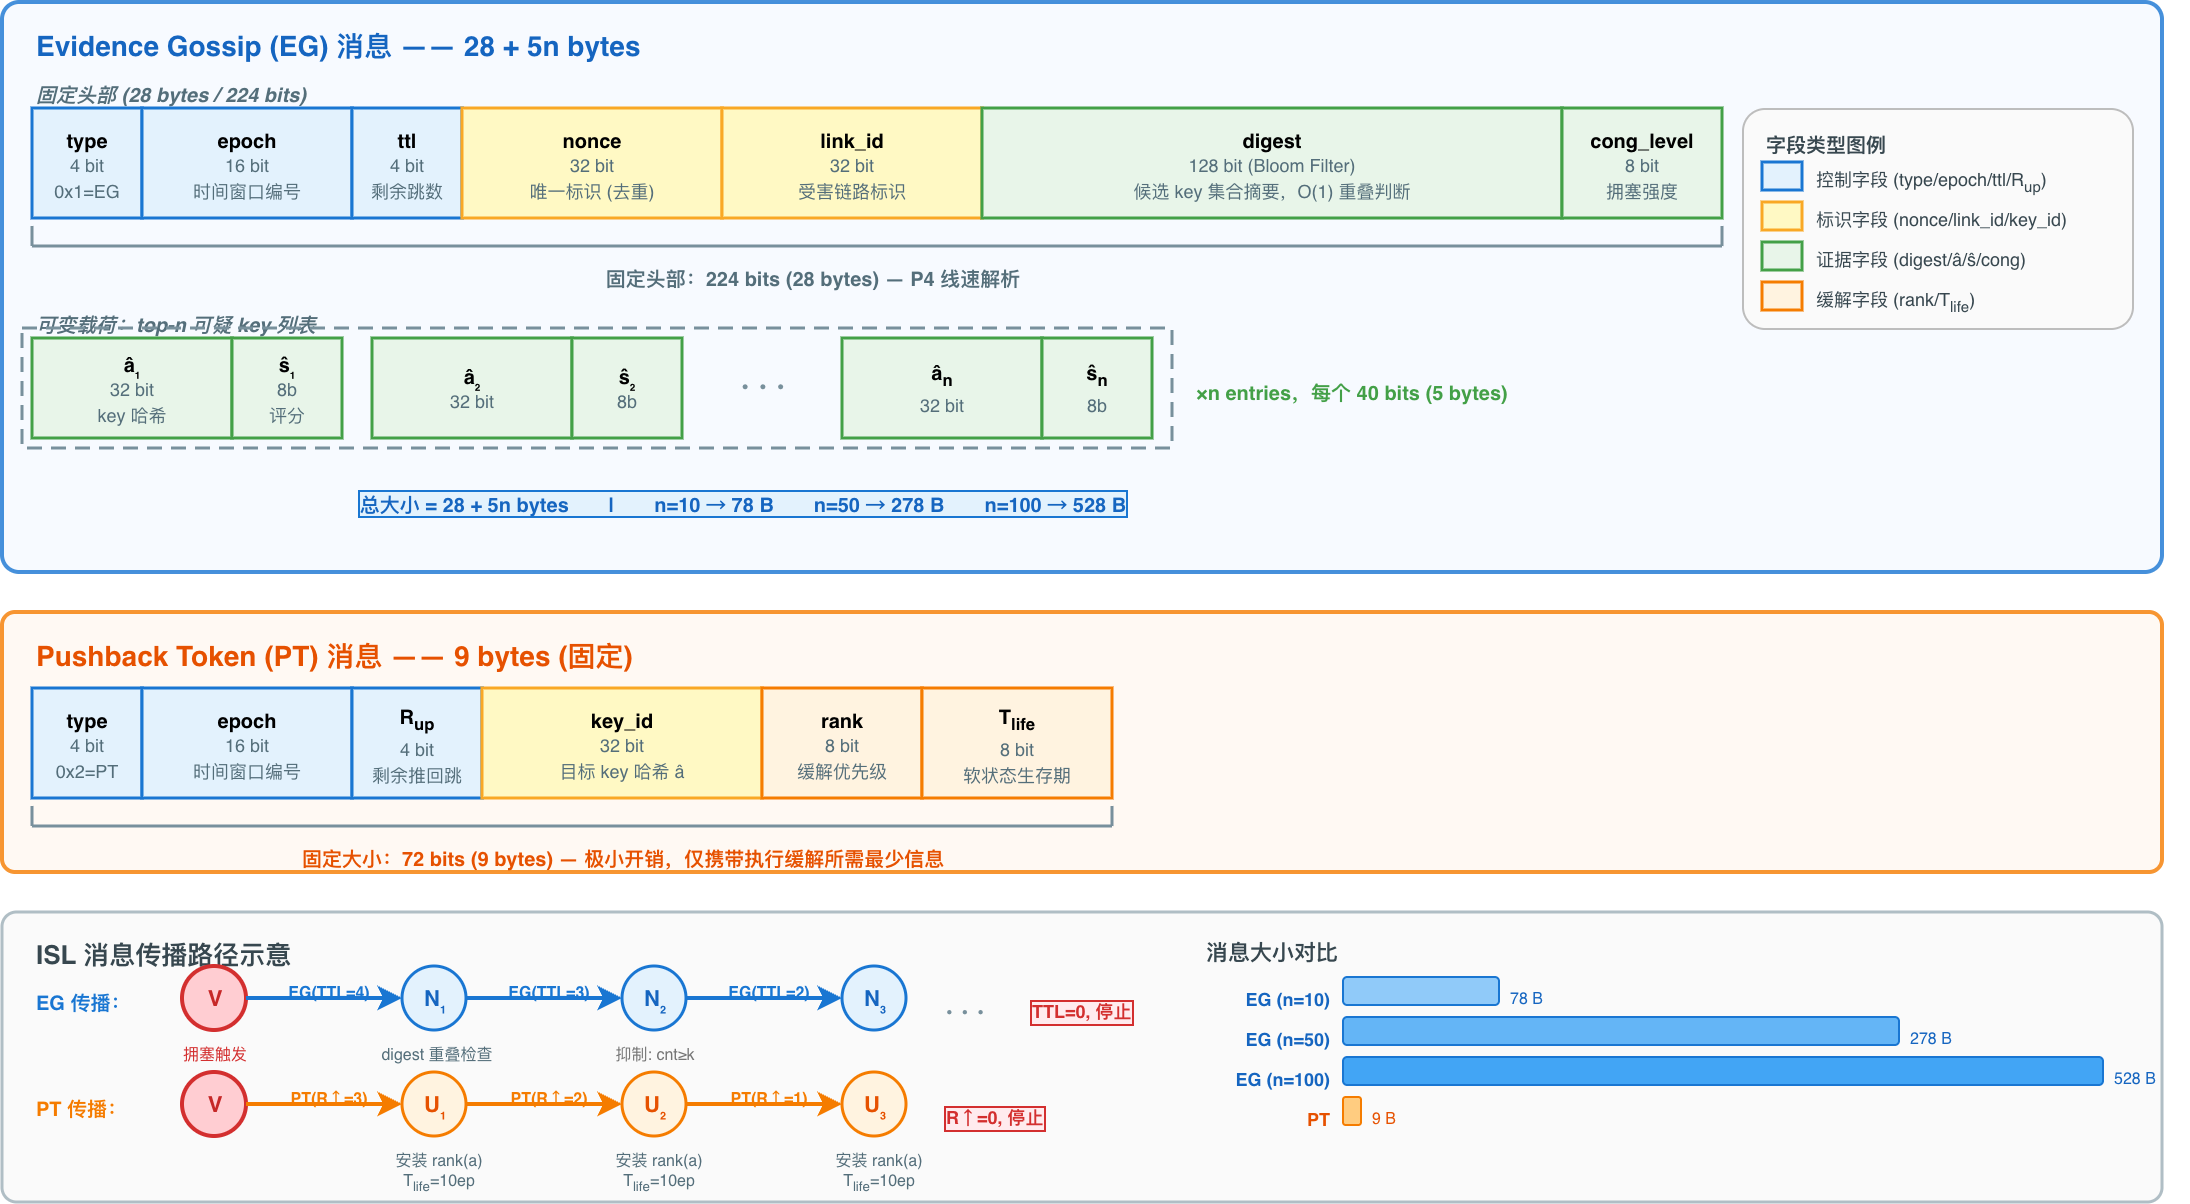
\includegraphics[width=0.92\linewidth]{figs/ch4/fig4_header.png}
\caption{\small 默认配置下的协同控制消息格式。上部：Evidence Gossip（EG）消息，固定头部 28~字节、可变载荷为 top-$n$ 可疑 key 列表，图中按默认 $n=10$ 绘制；字段按功能类型配色（蓝色=控制、黄色=标识、绿色=证据、橙色=缓解）。中部：Pushback Token（PT）消息，72~bit（9~字节）定长。下部：EG/PT 在 ISL 上的传播路径示意，以及默认 EG（$n=10$）与 PT 的消息大小对比。}
\label{fig:ch4_header}
\end{figure}

\subsubsection*{（3）抑制型扩散协议（Suppressed Gossip Protocol）}
设节点$v$在 epoch $\tau$内维护一个证据缓存$\mathcal{E}_{v,\tau}$，存储 ROI 内观察到的 EG 消息摘要。对任意$(\tau,\texttt{link\_id})$，节点以固定时隙$I = \Delta/4$执行一次抑制型扩散，即每个 epoch 内最多执行 4 轮扩散，且$I \ll \Delta$足以保证在 epoch 结束前完成收敛。其基本过程是：节点先在$I$内随机选择一个发送时刻$t_{\text{send}}$；若在$t_{\text{send}}$之前已经监听到至少$k$条等价证据（同一 epoch、同一 link\_id 且 digest 高度相似），则抑制本次发送；否则就在$t_{\text{send}}$发送聚合后的 EG 消息。通过随机化发送时机和冗余抑制，系统可以在保持传播速度的同时减少重复广播。

进一步地，为保证传播局部化，本章规定 EG 消息只有在满足相关性门限时才会继续转发。节点$v$收到来自邻居$u$的 EG 消息$M$后，计算其与本地候选集合$\mathcal{A}_{v,\tau}$的重叠度：
\begin{equation}
\Omega(M,v) = \frac{|\mathcal{A}_{v,\tau}\cap \mathcal{A}(M)|}{|\mathcal{A}(M)|},
\label{eq:overlap}
\end{equation}
其中$\mathcal{A}(M)$表示消息中的 top-$n$ key 集合。只有当$\Omega(M,v)\ge \theta_\Omega$或本地链路同样处于拥塞态$c_{v,e}(\tau)=1$时，节点才会将该证据纳入缓存并参与后续转发。这个机制借助本地观测的一致性过滤无关扩散，是控制信令规模的重要一环。

算法~\ref{alg:suppressed_gossip}给出了抑制型扩散协议的流程。与朴素 gossip 相比，这里的重点不在于能否传播，而在于结合物理网络的局部性和低度数结构，把传播范围控制在 ROI 内，并尽量避免同一证据在区域内反复回旋。

\begin{algorithm}[t]
\caption{抑制型邻居扩散协同（Suppressed Gossip Protocol）}
\label{alg:suppressed_gossip}
\Input{(1) 当前 epoch $\tau$ 的本地拥塞状态 $c_{v,e}(\tau)$ 与本地 EG 候选消息 $M_v$；\newline
(2) 节点状态：证据缓存 $\mathcal{E}_{v,\tau}$ 与发送窗口 $I$；\newline
(3) 协同参数：ROI 半径 $R$、抑制参数 $k$、重叠阈值 $\theta_\Omega$。}
\Output{节点本轮的发送结果 $O_v$：聚合 EG 消息 $\widetilde{M}_v$ 或抑制决策 \textsc{Suppress}。}
\BlankLine
\tcc{步骤 1：本地拥塞触发并启动抑制发送窗口}
初始化发送结果 $O_v\leftarrow \textsc{Suppress}$\;
若存在链路$e$使$c_{v,e}(\tau)=1$，构造本地EG候选消息$M_v$\;
将$M_v$加入缓存$\mathcal{E}_{v,\tau}$，并进入抑制发送窗口$I$\;
在窗口$I$内随机选择$t_{\text{send}}$\;
\BlankLine
\tcc{步骤 2：监听邻居消息并合并等价证据}
\While{$t < t_{\text{send}}$}{
    监听邻居EG消息$M_u$\;
    \If{$M_u$未去重（nonce未见过）且$M_u.\texttt{ttl}>0$}{
        计算$\Omega(M_u,v)$（可由digest快速近似）\;
        \If{$\Omega(M_u,v)\ge \theta_\Omega$ \textbf{or} 本地存在拥塞链路}{
            将$M_u$合并入$\mathcal{E}_{v,\tau}$（top-$n$合并$+$digest并集）\;
        }
    }
}
统计窗口$I$内等价证据数量$cnt$\;
\BlankLine
\tcc{步骤 3：根据冗余程度决定转发或抑制}
\eIf{$cnt < k$}{
    生成聚合消息$\widetilde{M}_v = \texttt{Aggregate}(\mathcal{E}_{v,\tau})$\;
    设置$\widetilde{M}_v.\texttt{ttl}\leftarrow \min(\texttt{ttl}_{\text{received}}-1,\, R)$，向所有邻居发送（不回发原入端口）\;
    $O_v\leftarrow \widetilde{M}_v$\;
}{
    抑制发送（suppress）\;
}
\textbf{return} $O_v$\;
\end{algorithm}

\noindent\textbf{\texttt{Aggregate}策略说明。}函数$\texttt{Aggregate}(\mathcal{E}_{v,\tau})$对缓存中的所有 EG 消息执行如下合并：（i）同一 key $a$若出现在多条消息中，则取$\widehat{s}(a) = \max_j \widehat{s}_j(a)$，保留最强证据；（ii）对 digest 按位 OR，得到 Bloom Filter 摘要并集，保证接收端能够判断聚合后候选集的覆盖范围；（iii）若合并后的 key 集合超过$n$，则按$\widehat{s}(a)$降序保留前$n$个，保证消息大小恒定。这样处理后，消息仍然紧凑，同时优先传播高置信度证据。

\noindent\textbf{TTL收敛性保证。}算法~\ref{alg:suppressed_gossip}中的聚合发送步骤采用$\texttt{ttl}\leftarrow \min(\texttt{ttl}_{\text{received}}-1, R)$，从而保证每次转发时 TTL 至少递减 1，即使经过聚合节点也不会被重置为完整 TTL。因此，在$R$跳半径的 ROI 内，消息最多经历$R$次转发后就会终止，不存在无限传播风险。

\subsection{协同判定与推回缓解：从受害链路推回到上游入口}
\label{subsec:ch4_pushback}

\subsubsection*{（1）协同证据聚合与判定}
在ROI内，多个节点对同一攻击相关key会给出不同程度的本地评分$S_{v,\tau}(a)$。为形成网络级判定，本章定义协同聚合评分：
\begin{equation}
S^{\text{net}}_{\tau}(a) = \sum_{v\in \mathcal{R}_{\tau}}\omega_v \cdot \widetilde{S}_{v,\tau}(a),
\label{eq:net_score}
\end{equation}
其中$\mathcal{R}_{\tau}$为在epoch $\tau$内参与协同的ROI节点集合，$\widetilde{S}_{v,\tau}(a)$为归一化后的本地评分，$\omega_v$为权重。权重的设计根植于物理可观测量：拥塞越强、越接近受害链路的节点，其证据应更可靠。于是本章取：
\begin{equation}
\omega_v = \frac{\left(1+\lambda\cdot \texttt{cong\_level}_v\right)\cdot \exp(-\mu\cdot \texttt{dist}(v,e^\*))}{\sum_{u\in\mathcal{R}_\tau}\left(1+\lambda\cdot \texttt{cong\_level}_u\right)\cdot \exp(-\mu\cdot \texttt{dist}(u,e^\*))},
\label{eq:weight}
\end{equation}
其中$\texttt{dist}(v,e^\*)$表示$v$到受害链路$e^\*$的跳数距离，$\lambda,\mu$为超参数，且所有参与节点的权重满足$\sum_{v\in\mathcal{R}_\tau}\omega_v = 1$。$\lambda$控制拥塞等级对权重的放大程度，$\mu$控制距离衰减速率。实现时，为避免复杂指数运算，控制面 agent 采用查表或分段线性近似完成权重计算；数据面只需提供$\texttt{cong\_level}$与邻接关系。式\eqref{eq:net_score}在本章中的主要用途是让 pushback 触发更稳定。它通过汇总 ROI 内的局部证据来压制单节点的瞬时误判，避免某处偶发异常立刻触发全区域推回。在后文的均匀 bot 分布实验中，CoopSatShield 与 MS-SatShield 的检测 F1 保持一致，因此本章的证据更支持把它理解为网络级触发融合机制，而不是证明加权聚合在检测能力上一定优于简单的 max 或 avg 规则。

推回判定阈值$\Theta_{\text{pb}}$的选取遵循如下工程原则：在预设验证场景下（含$M=10,50,100$三组碎片化设定），控制误推回率（即良性key被触发推回的概率）不超过$5\%$，并在此约束下选择一组稳定的触发工作点。后续实验统一采用$\Theta_{\text{pb}}=0.7$、$\lambda=1.0$、$\mu=0.5$。由于本章尚未单列weighted / unweighted / max三类聚合规则的消融对比，这些参数应理解为可工作的默认配置，而非全局最优解。

当存在$a$使$S^{\text{net}}_{\tau}(a)\ge \Theta_{\text{pb}}$时，系统对该key触发推回缓解；若多个key满足条件，则按$S^{\text{net}}_{\tau}(a)$排序取前$n_{\text{pb}}$个执行，以保证数据面策略表规模可控。

\subsubsection*{（2）推回令牌（PT）与逐跳传播}
pushback 的重点在于，它不依赖全局路由逆推，而是利用逐跳可观测的上游贡献来实现近似反向路径传播。具体来说，受害链路附近节点$v$对 key $a$计算其入端口贡献分布$\pi_{v,\tau}(a,p)$（式\eqref{eq:ingress_contrib}），再选择贡献最大的前$r=\min(2,d-1)$个上游端口集合$\mathcal{P}^\uparrow_{v}(a)$；在$d=4$的 LEO ISL 结构中，$r=2$。随后，节点向对应上游邻居发送 PT 令牌。令牌携带软状态生存期$T_{\text{life}}$与剩余推回跳数$R_{\uparrow}$，上游节点收到后立即在本地数据面安装短时效缓解规则，如队列降权或限速，并继续沿相同思路向更上游传播。由于 LEO 网络连接度较低、拓扑变化发生在秒级\citess{icarus}，这种逐跳机制在每个 epoch 内都具有稳定语义；同时，软状态到期后会自动失效，从而避免拓扑变化后留下过期规则。

算法~\ref{alg:pushback}给出了pushback传播流程。

\begin{algorithm}[t]
\caption{逐跳推回缓解（Hop-by-hop Pushback）}
\label{alg:pushback}
\Input{(1) 触发 key 集合 $\mathcal{A}^{\text{pb}}_\tau$ 及其缓解等级 $\texttt{rank}(a)$；\newline
(2) 各节点的入端口贡献分布 $\pi_{v,\tau}(a,p)$ 与本地软状态规则表；\newline
(3) 推回参数：推回半径 $R_{\uparrow}$、上游分支数 $r$、软状态生存期 $T_{\text{life}}$。}
\Output{本地安装或刷新的缓解规则，以及继续向上游传播的 PT 令牌集合 $\mathcal{T}^{\uparrow}$。}
\BlankLine
\tcc{步骤 1：受害节点按入端口贡献选择上游并发起 PT}
初始化待转发 PT 集合 $\mathcal{T}^{\uparrow}\leftarrow\varnothing$\;
\ForEach{$a\in\mathcal{A}^{\text{pb}}_\tau$}{
    在节点$v$生成PT令牌：$\langle a,\, \texttt{rank},\, \tau,\, R_{\uparrow},\, T_{\text{life}}\rangle$\;
    计算上游贡献分布$\pi_{v,\tau}(a,p)$，选取前$r$大端口$\mathcal{P}^\uparrow_v(a)$\;
    向$\mathcal{P}^\uparrow_v(a)$对应邻居发送PT\;
    将对应 PT 记入 $\mathcal{T}^{\uparrow}$\;
}
\BlankLine
\tcc{步骤 2：上游节点安装软状态并递归继续推回}
\eIf{PT未过期且$R_{\uparrow}>0$}{
    在本地数据面安装/刷新软状态规则：$\texttt{rank}(a)\leftarrow$ PT.$\texttt{rank}$，有效期$T_{\text{life}}$\;
    $R_{\uparrow}\leftarrow R_{\uparrow}-1$\;
    基于$\pi_{u,\tau}(a,\cdot)$继续向上游前$r$大邻居传播\;
    将更新后的 PT 记入 $\mathcal{T}^{\uparrow}$\;
}{
    丢弃该 PT\;
}
\textbf{return} 本地安装或刷新的缓解规则，以及继续向上游传播的 PT 令牌集合 $\mathcal{T}^{\uparrow}$\;
\end{algorithm}

\noindent\textbf{rank到队列映射与限速动作。}PT中的$\texttt{rank}$字段映射到三级缓解强度：（i）$\texttt{rank}=\text{High}$：匹配key的流量被调度至最低优先级队列Queue~0，带宽上限设为链路容量的$5\%$，实现近乎完全阻断；（ii）$\texttt{rank}=\text{Med}$：调度至Queue~1，带宽上限为$20\%$；（iii）$\texttt{rank}=\text{Low}$：调度至Queue~2，仅降低调度优先级但不硬限速。数据面通过match-action表项实现：以key哈希$\widehat{a}$匹配入向流量，命中后修改队列标记字段并施加对应meter速率。当同一key在同一epoch内收到多个PT（来自不同下游节点或路径），取最严格的rank值（即$\text{High} > \text{Med} > \text{Low}$）；若新PT的rank弱于已安装规则，则忽略。跨epoch时，新PT刷新$T_{\text{life}}$计时器，确保软状态的时效性。

图~\ref{fig:ch4_pushback}直观展示了上述推回过程的完整生命周期。该图分为三个阶段：

\textbf{阶段1}（图左上角）展示受害节点$V$的拥塞检测过程：数据面检测到受害链路$e^*$的队列占用超过阈值（$q_{v,e^*}>Q_\text{th}$，即$c(v,e^*)=1$），并输出top-$K$候选key的入端口贡献分布$\pi(a_1,p)$。图中小型条形图显示key $a_1$在三个入端口的贡献比例分别为$70\%$、$20\%$和$10\%$，指明主攻击方向。当协同聚合评分$S^\text{net}(a_1)=0.87\ge\Theta_\text{pb}=0.7$时，系统触发推回。

\textbf{阶段2}（图中部）展示PT令牌的逐跳反向传播。受害节点$V$生成PT$=\langle a_1, \texttt{rank}=\text{High}, \tau, R_\uparrow=3, T_\text{life}=10\rangle$，选择贡献最大的前$r=2$个上游端口（$p_1$: $65\%\rightarrow U_1$，$p_2$: $20\%\rightarrow U_1'$），向对应邻居发送PT。各接收节点（$U_1, U_1'$）立即在本地数据面安装软状态缓解规则$\texttt{rank}(a_1)\leftarrow\text{High}$，并将$R_\uparrow$递减后继续向上游传播。经过3跳后$R_\uparrow=0$，传播终止于节点$U_3, U_3'$。图中金色shield图标标注了所有已安装缓解规则的节点，绿色渐变链路标注了推回释放的带宽。

\textbf{阶段3}（图右下角）定量对比推回前后的效果：按本文统一采用的路径积分无效占用成本口径，推回前攻击流经历$h=5$跳到达$e^*$，$W_\text{waste}=\text{rate}\times5$；推回后攻击流在$U_3$处被限速/丢弃（$h=2$跳），$W_\text{waste}=\text{rate}\times2$，降低$60\%$。图右上角的时间线展示了软状态生命周期$T_\text{life}$：PT在epoch $\tau$安装后持续生效$T_\text{life}=10$个epoch，到期自动清除；若攻击仍在持续，新一轮PT将刷新规则，避免拓扑变化后产生"幽灵规则"。

\begin{figure}[!htb]
\centering
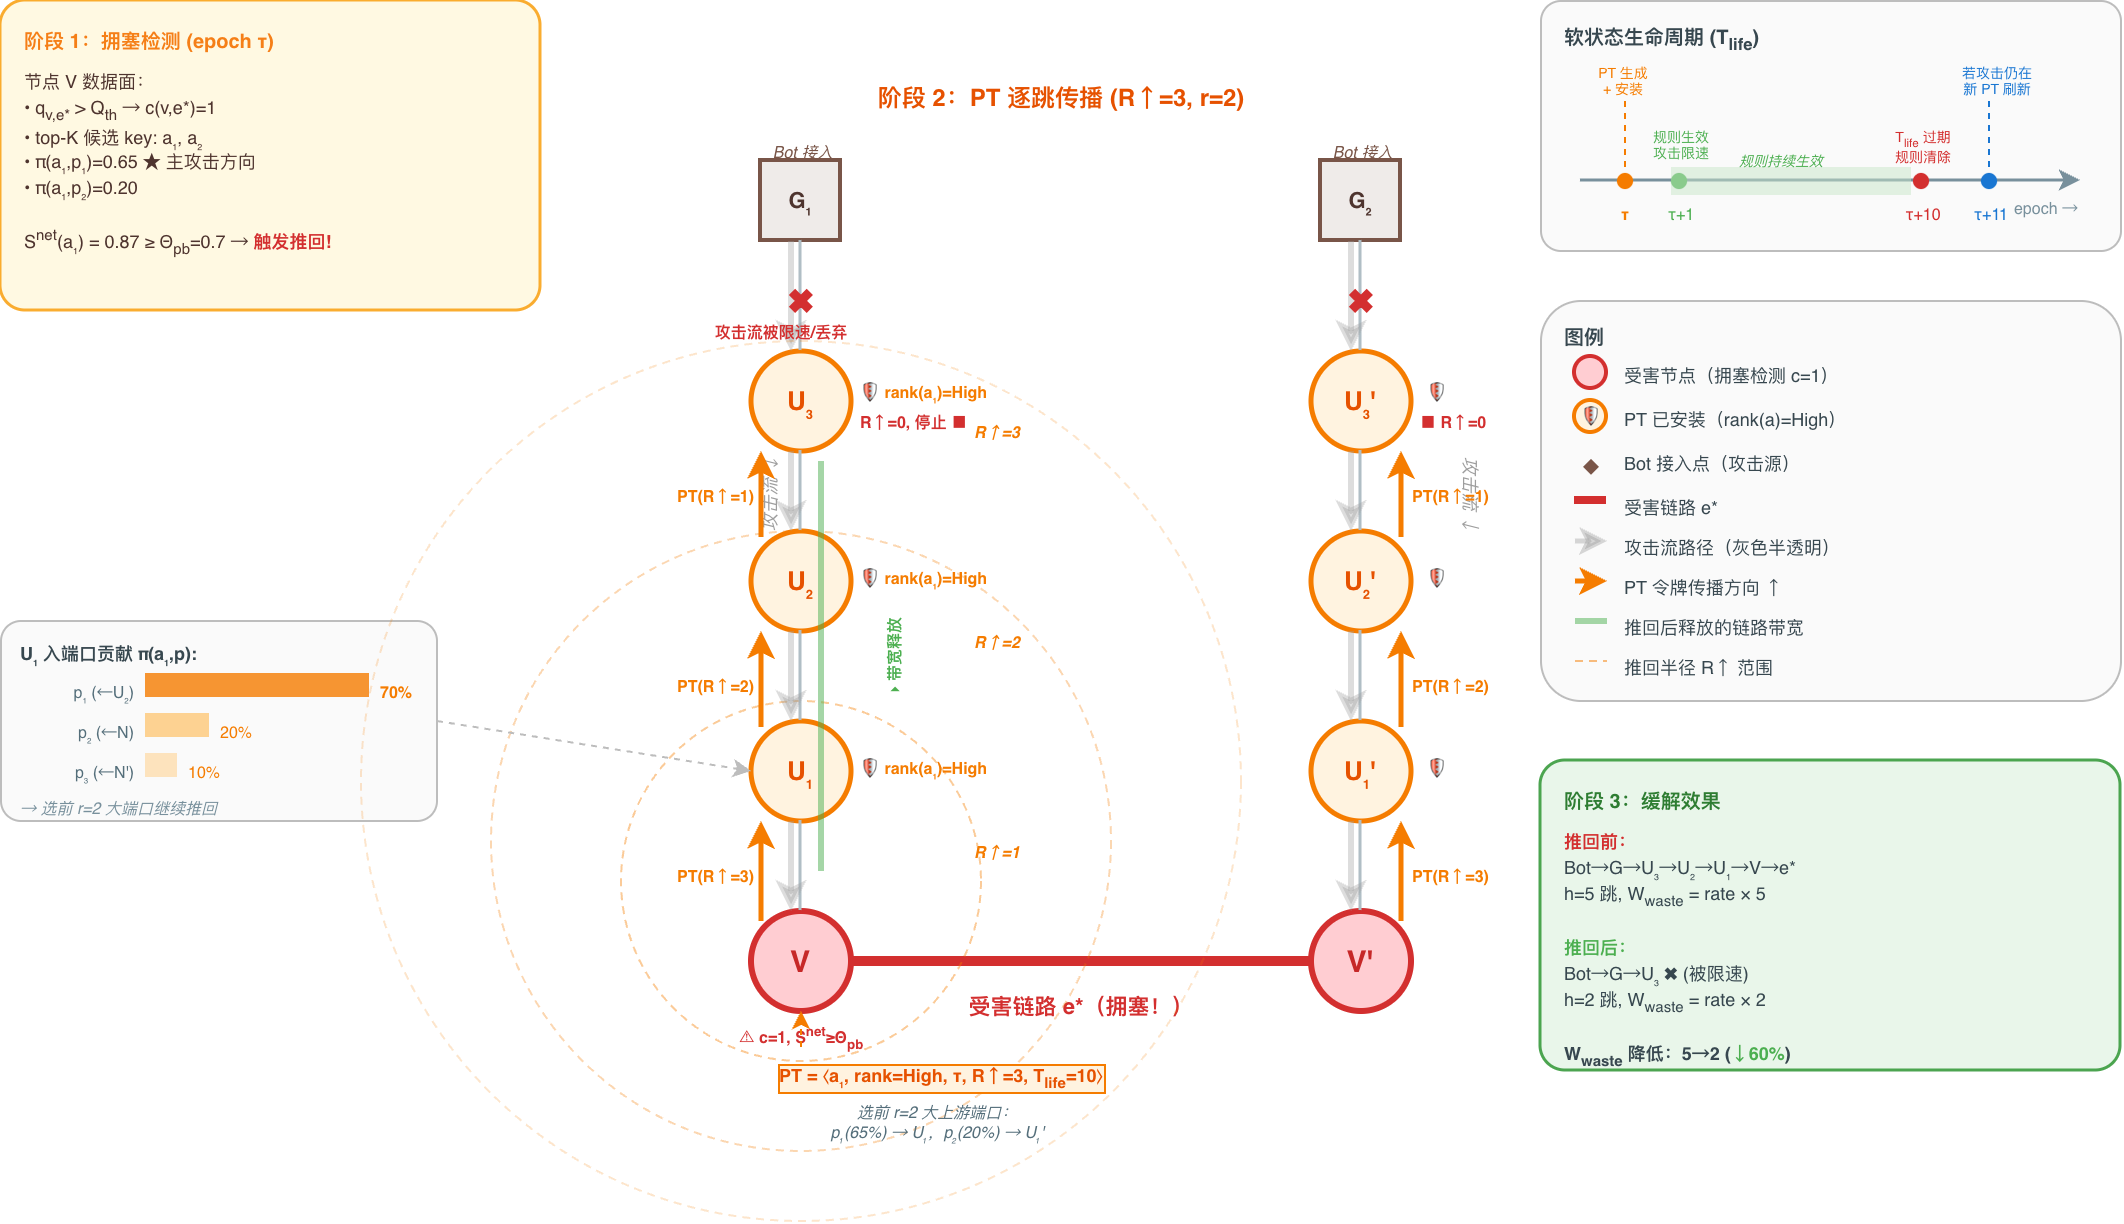
\includegraphics[width=0.93\linewidth]{figs/ch4/fig4_pushback.png}
\caption{\small 逐跳推回缓解传播示意。左上：阶段1——拥塞检测与入端口贡献分布$\pi(a,p)$；中部：阶段2——PT令牌从受害链路$e^*$向上游逐跳扩散（$R_{\uparrow}=3$，$r=2$分支），沿途节点安装软状态缓解规则；右下：阶段3——推回前后的$W_{\text{waste}}$对比（$h$从5跳降至2跳）。右上：软状态生命周期$T_{\text{life}}$时间线。}
\label{fig:ch4_pushback}
\end{figure}

\subsection{信令开销与可实现性分析}
\label{subsec:ch4_overhead}

\subsubsection*{（1）ROI限制下的信令规模上界}
设星座网络的平均度数为$d$（典型LEO ISL结构中$d\approx4$）\citess{icarus}。对任意EG消息，TTL为$R$时，其在最坏情况下可触达的节点数不超过一个$d$叉树的$R$层节点规模：
\begin{equation}
| \text{ROI}(R) | \le 1 + d\cdot \frac{(d-1)^R - 1}{d-2},\quad d>2.
\label{eq:roi_bound}
\end{equation}
当$d=4$时，上界为$| \text{ROI}(R) | \le 2\cdot 3^R -1$。例如$R=4$时，最坏触达规模不超过161个节点，远小于Starlink Shell 1的1584节点总规模\citess{icarus}。因此，TTL本身已经把协同传播限制在受影响的局部区域内，避免全网泛洪。

\subsubsection*{（2）抑制机制下的消息量与带宽开销}
在抑制型扩散中，节点在一个发送窗口内若监听到不少于$k$条等价证据即抑制发送，从而大幅降低重复广播。对\emph{单个协同事件}$(\tau,\texttt{link\_id})$而言，设ROI内有效参与节点数为$N_R$，且每个节点在该事件上每epoch至多发送一次聚合EG消息，则EG消息总数满足：
\begin{equation}
M_{\text{EG}}(\tau,\texttt{link\_id}) \le N_R.
\label{eq:msg_count}
\end{equation}
进一步地，若该事件对应的EG与PT消息大小分别为$L_{\text{EG}}$、$L_{\text{PT}}$字节，PT消息数为$M_{\text{PT}}(\tau,\texttt{link\_id})$，则其单事件控制带宽开销上界为：
\begin{equation}
B_{\text{ctrl}}^{(\tau,\texttt{link\_id})} \le \frac{M_{\text{EG}}(\tau,\texttt{link\_id})\cdot L_{\text{EG}} + M_{\text{PT}}(\tau,\texttt{link\_id})\cdot L_{\text{PT}}}{\Delta}.
\label{eq:ctrl_bw}
\end{equation}
若同一epoch内同时出现多条独立拥塞链路，则总控制开销可写为对所有事件的求和。结合式\eqref{eq:roi_bound}与Starlink ISL 20~Gb/s容量级\citess{icarus}，当$R$取小常数（本章默认$R=4$）时，$B_{\text{ctrl}}$相对ISL带宽占比可控制在远低于$1\%$的量级。实验中我们进一步验证了控制开销与$R,k,\Delta$的敏感性（见第\ref{subsec:ch4_results}节），并观察到抑制机制使得在攻击高峰期也不会出现信令风暴。

\subsubsection*{（3）数据面实现可行性}
实现上，本章遵循数据面负责常数复杂度快路径、控制面负责聚合与决策的分工。数据面新增逻辑主要包括协同消息的轻量 header 解析与 TTL 递减、seen-set 去重（可由 Bloom Filter 近似实现）、key 的入端口贡献统计$\text{bytes}_{v,\tau}(a,p)$，以及 pushback 规则的执行与软状态清理。这些操作都可以由可编程交换机的寄存器阵列与 match-action 表实现\citess{bosshart2013rmt}，每包处理仍保持 O(1) 复杂度，满足线速约束。复杂的聚合评分（式\eqref{eq:net_score}）和抑制决策则交由星上 agent 完成，避免数据面承担过重计算负担。

\section{仿真与分析}
\label{sec:ch4_eval}

\subsection{实验设置}
\label{subsec:ch4_setup}

本章的仿真实验基于自研 Python 仿真框架实现（与\ref{chap:ms_satshield}相同）。该框架集成了星座拓扑构建、最短路计算、epoch 级事件驱动与数据面行为模拟，拓扑构建与路由策略参考 Hypatia 仿真平台\citess{hypatia}的快照路由模型\citess{handley2019delay}。评估采用 Starlink Shell 1 拓扑，该拓扑包含 1584 颗卫星（72 轨道面$\times$22 颗/面），ISL 为典型的 4 链路连接结构，ISL 带宽 20~Gb/s，上下行链路容量为数 Gb/s 量级\citess{icarus}。epoch 长度取$\Delta=1$~s，与卫星拓扑快照更新周期对齐\citess{icarus}。表~\ref{tab:ch4_params}汇总了本章实验使用的主要参数。为贴近真实网络背景流量，本文采用 CAIDA UCSD Anonymized Internet Traces 2018 数据集（OC-192 链路，采集于 Equinix-Chicago 监测点）构造良性流量：原始 trace 按比例缩放至 20~Gb/s ISL 容量级别，并按人口加权的城市对分布模型将源-目的 IP 映射到 LEO 地面终端对，映射参数与\ref{chap:ms_satshield}中的设置一致\citess{satshield}。攻击流量则采用 ICARUS 式 LFA 策略生成，攻击者利用公开轨道与拓扑信息选择 bot 对并计算使目标链路拥塞的流量分配\citess{icarus}；同时，在更强的对手模型下引入低速化、多 decoy、脉冲化和滚动目标等策略，用来检验协同机制对碎片化证据的聚合能力。

为避免实验设置中声明的指标多于正文实际汇报的指标，本章只报告与后续图表直接对应的四类结果：路径积分无效带宽占用成本$W_{\text{waste}}$（单位 Mb/s$\cdot$hop，对应式\eqref{eq:waste_bw}）；攻击期间的良性吞吐，以及两类响应时延，本地检测生效时延$T_{\text{det}}=t_{\text{first-local-rule}}-t_{\text{attack-start}}$和 pushback 生效时延$T_{\text{pb}}=t_{\text{first-pushback-rule}}-t_{\text{attack-start}}$；检测质量，即攻击相关 key 识别的 Precision、Recall 和 F1（定义同\ref{chap:ms_satshield}式( \ref{eq:f1_def} )）；以及协同开销，即 EG/PT 消息数与字节开销。除非特别说明，下文提到的吞吐都指攻击持续阶段的 epoch 平均值，不包含 warmup 与恢复段。

\begin{table}[t]
\centering
\caption{第四章实验主要参数设置}
\label{tab:ch4_params}
\begin{tabular}{l|l|l}
\hline
参数 & 含义 & 取值 \\
\hline
$\Delta$ & epoch长度 & 1~s \\
$I$ & 抑制扩散时隙 & $\Delta/4 = 0.25$~s \\
$R$ & ROI半径（EG TTL） & 4跳 \\
$R_{\uparrow}$ & 推回半径（PT跳数） & 3跳 \\
$k$ & 抑制参数 & 3 \\
$n$ & EG携带的top-$n$ key数 & 10（默认）；图~\ref{fig:ch4_ctrl_overhead}(b)按保守$n=100$计费 \\
$r$ & 推回上游分支数 & $\min(2,d-1)=2$ \\
$\theta_\Omega$ & 相关性门限 & 0.3 \\
$Q_{\text{th}},D_{\text{th}}$ & 拥塞告警阈值 & 继承第\ref{chap:ms_satshield}章部署配置（本章不单独调参） \\
$\Theta_{\text{pb}}$ & 推回判定阈值 & 0.7 \\
$\lambda$ & 拥塞权重放大因子 & 1.0 \\
$\mu$ & 距离衰减因子 & 0.5 \\
$T_{\text{life}}$ & PT软状态生存期 & 10 epoch \\
\hline
\end{tabular}
\end{table}

\begin{table}[t]
\centering
\caption{量化对比基线设置（第四章正文结果）}
\label{tab:ch4_baselines}
\begin{tabular}{l|l}
\hline
方案 & 说明 \\
\hline
NoDefense & 无防御，FIFO/ECMP默认转发 \\
SatShield & 单星top-$k$过滤+队列调度缓解\citess{satshield} \\
MS-SatShield & \ref{chap:ms_satshield}多签名增强，但无协同/无pushback \\
\textsc{CoopSatShield} & 本章方案：抑制型扩散协同+逐跳pushback \\
\hline
\end{tabular}
\end{table}

表~\ref{tab:ch4_baselines}中的四种方案构成了本章正文图表的量化比较范围。至于 LinkScope、Woodpecker、RADAR、Ripple 与 Mew 等典型地面 LFA 防御机制\citess{linkscope,woodpecker,radar,ripple,mew}，本文仍将其作为相关工作与设计参照。它们分别代表主动测量、集中式流量工程、相关性检测和可编程数据面分布式防御等不同技术路线，但由于这些方案依赖的控制闭环、硬件资源或拓扑稳定性假设与 LEO 场景差异明显，本章尚未在统一的 LEO 仿真口径下完成等价复现，因此不把它们写成正文中的数值基线，也不据此宣称实验优势。若后续补齐统一实现，更合适的呈现方式应是一张代表场景下的指标汇总表，而不是继续堆叠多条长曲线。

\subsection{结果与分析}
\label{subsec:ch4_results}

\subsubsection*{（1）推回缓解带来的网络级收益}
图~\ref{fig:ch4_waste_reduction}以分组柱状图展示了在不同碎片化程度$M\in\{1,10,100,1000\}$下，各方案对路径积分无效带宽占用成本$W_{\text{waste}}$的影响。实验结果可以分为三种情形来看。

当$M\leq10$时，SatShield与MS-SatShield表现接近，均可将$W_{\text{waste}}$降至 NoDefense 的$7.2\%$（$M=1$）和$19.8\%$（$M=10$）。这是因为此时攻击 key 的聚合速率远高于良性长尾，rate-only 已能稳定检出，多签名不会带来额外增益。CoopSatShield 则通过推回把丢弃位置继续前移到上游$R_{\uparrow}=3$跳附近，使$W_{\text{waste}}$在$M=1$时进一步降到$3.0\%$。这里的收益主要来自 pushback 缩短攻击流实际承载路径，而不是协同证据聚合；在$M=1$时，单节点已经足以检出唯一的攻击 key。这说明即使不存在明显碎片化，pushback 本身也具有独立的带宽节约价值。

当$M=100$时，SatShield 的 rate-only 检测已经基本失效（F1$=0.017$），$W_{\text{waste}}=248{,}995$~Mb/s$\cdot$hop，与 NoDefense 的$251{,}005$只差$0.8\%$，几乎等同于无防御。这一结果与\ref{chap:ms_satshield}图~\ref{fig:ch3_fig2_f1}(b)中的分离段分析一致，因为在$M=100$时速率特征已经落入良性长尾。MS-SatShield 依靠 FO/FI 特征仍能保持有效检测（F1$=0.909$），使$W_{\text{waste}}$降至 NoDefense 的$17.1\%$；CoopSatShield 再通过推回把这一比例进一步压低到$11.0\%$，相较 MS-SatShield 额外释放了$6.1$个百分点的链路带宽。

当$M=1000$时，攻击 key 大量脱离 top-$K$候选集（TopK~Recall$\approx0.30$），所有方案的$W_{\text{waste}}$都明显上升。MS-SatShield 与 CoopSatShield 仍然优于 SatShield，分别占 NoDefense 的$72.5\%$和$70.8\%$，但改善幅度已经有限，这反映的正是\ref{chap:ms_satshield}中指出的候选集覆盖率瓶颈。

这些结果与式\eqref{eq:waste_bw_approx}描述的推回收益机理是一致的，即推回把攻击流的平均承载跳数$\bar h$从完整路径长度压缩到$R_{\uparrow}$跳量级。同时，不同$M$值下的渐进退化设定也延续了\ref{chap:ms_satshield}中的分析路径：先是 rate-only 仍然有效，再到需要多签名补偿，最后进入候选集覆盖率受限的区间。

\begin{figure}[!htb]
\centering
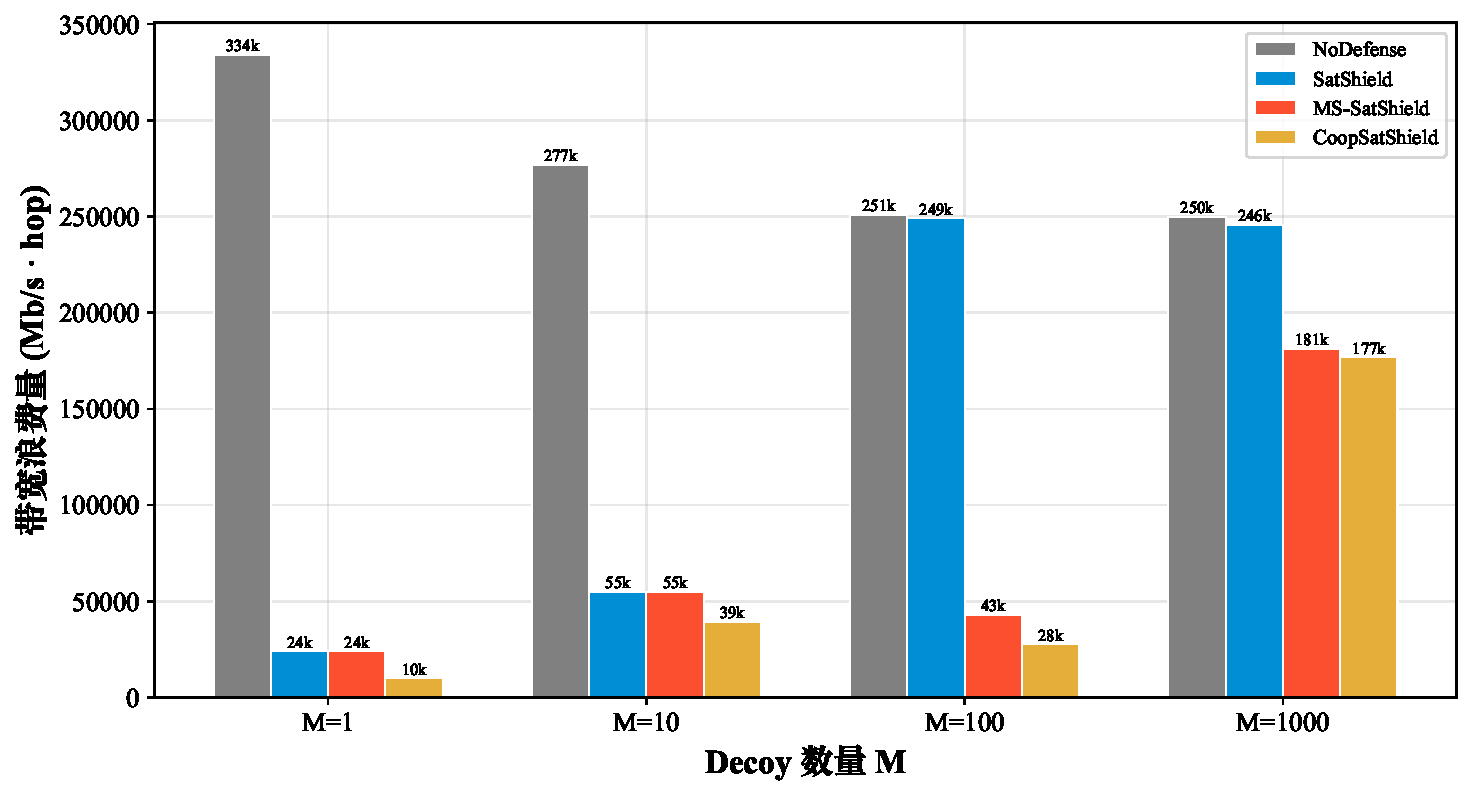
\includegraphics[width=0.92\linewidth]{figs/ch4/fig4_waste.pdf}
\caption{不同碎片化程度$M$下的无效带宽占用$W_{\text{waste}}$对比。四组分组柱状图分别对应$M=1,10,100,1000$，每组包含NoDefense（灰）、SatShield（蓝）、MS-SatShield（红）、CoopSatShield（金）四种方案，柱顶标注具体数值。}
\label{fig:ch4_waste_reduction}
\end{figure}

\subsubsection*{（2）良性吞吐与反应时间}
图~\ref{fig:ch4_throughput}给出了$M=100$攻击场景下良性吞吐随时间（epoch）变化的全过程。实验将攻击窗口设置为 epoch~30 至 epoch~120（共 90 个 epoch），图中粉色背景标出攻击持续阶段，竖虚线分别对应攻击开始、首次检测和推回生效三个时刻。按上一节的定义，本地检测生效时延为$T_{\text{det}}=1$~epoch，pushback 生效时延为$T_{\text{pb}}=2$~epoch。

\textbf{攻击前}（epoch~0$\sim$29），所有方案的良性吞吐都稳定在 1.0 附近，符合网络正常运行状态。

\textbf{攻击触发与检测延迟}（epoch~30）：由于检测算法至少需要 1 个 epoch 的统计积累，攻击开始后的第一个 epoch 内所有方案都无法检出攻击流，良性吞吐统一跌至 NoDefense 水平$\approx0.71$。这一短暂下探反映的是在网检测的内在时滞，对所有基线都成立。

\textbf{首次检测生效}（epoch~31）：SatShield 的 rate-only 检测在$M=100$下完全失效（F1$=0.017$），因此吞吐仍维持在 NoDefense 水平。MS-SatShield 依靠多签名检测能力（F1$=0.909$），通过高优先级队列保留机制（80\% 带宽保留）将攻击期间的良性吞吐恢复到$0.886$，相对 NoDefense 提升了$17.5$个百分点。CoopSatShield 在这一时刻暂时与 MS-SatShield 处于同一水平，因为检测已经生效，但推回尚未传播完成。

\textbf{推回生效}（epoch~32+）：当 gossip 消息完成 ROI 内扩散后，CoopSatShield 的 pushback 规则开始在上游节点生效，约$86\%$的已检测攻击流在上游被直接丢弃，中间链路带宽因此得到释放。稳态下，CoopSatShield 的吞吐恢复至$0.959$，相较 MS-SatShield 进一步提升了$7.3$个百分点。由于推回覆盖率并未达到$100\%$，仍有约$14\%$的攻击流沿非推回路径到达目标链路，因此稳态吞吐停留在$0.959$而不是理想的$1.0$，这体现了分布式推回在工程实现上的实际边界。

\textbf{攻击结束}（epoch~120后）：所有方案的吞吐都迅速恢复到$1.0$附近。整体来看，CoopSatShield 的吞吐恢复表现为两个连续阶段：先由检测触发的队列调度提供基础保护（$+17.5$~pp），再由推回带来的上游丢弃继续提供增量收益（$+7.3$~pp），最终使良性吞吐在攻击期间稳定维持在约$0.96$。

\begin{figure}[!htb]
\centering
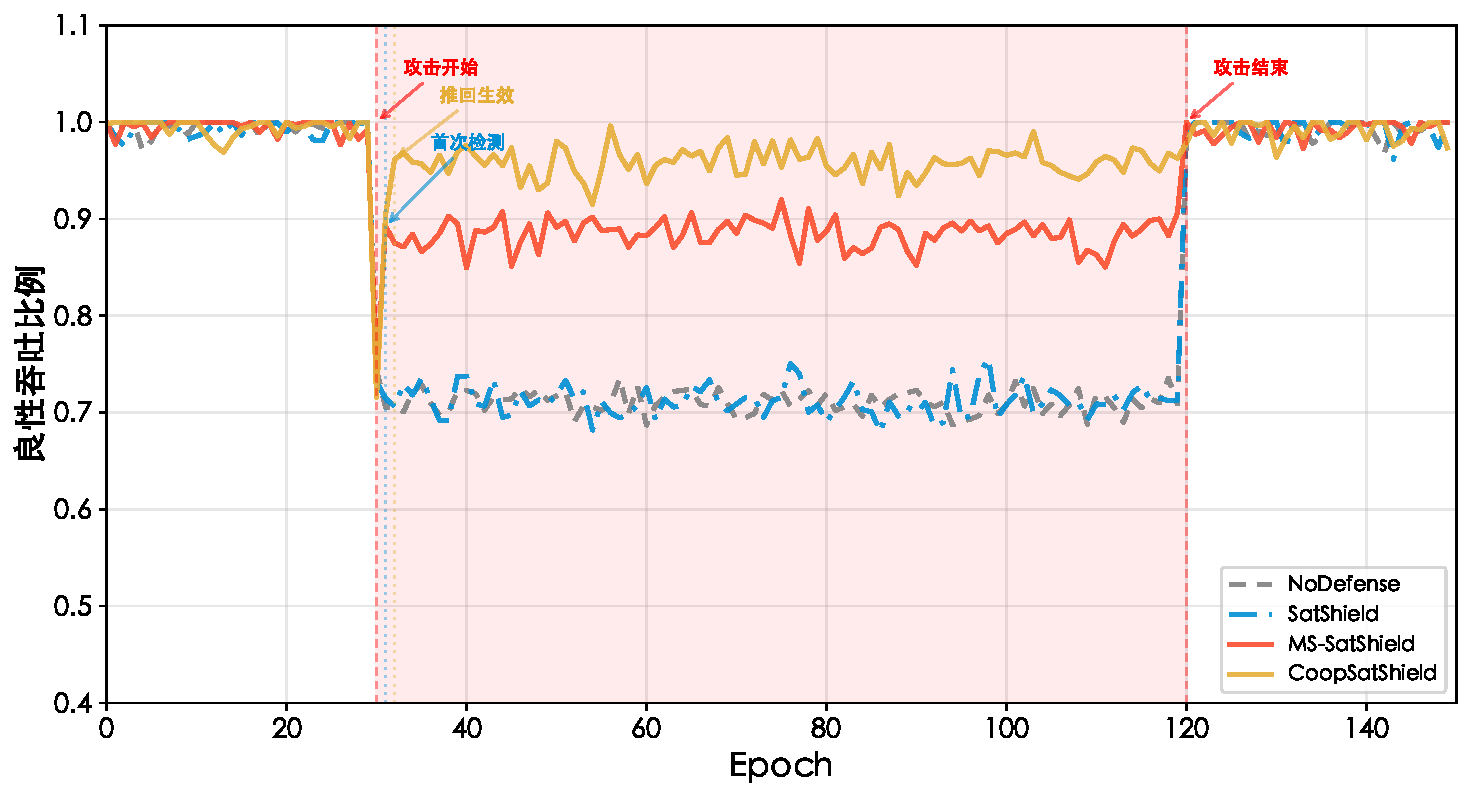
\includegraphics[width=0.92\linewidth]{figs/ch4/fig4_throughput.pdf}
\caption{良性吞吐随时间变化（$M=100$）。粉色背景标注攻击持续阶段（epoch~30$\sim$120），竖虚线分别对应攻击开始、首次检测与推回生效三个时刻。CoopSatShield经历两步递升：检测恢复至0.89，推回进一步至0.96。}
\label{fig:ch4_throughput}
\end{figure}

\subsubsection*{（3）协同开销与无信令风暴验证}
本章最关心的工程风险之一，是大规模网络中的信令风暴。图~\ref{fig:ch4_ctrl_overhead}用$1\times3$子图展示了协同开销和抑制机制的效果。

子图~(a)比较了有抑制（$k=3$）和无抑制两种情况下，EG 消息数随 ROI 半径$R$的变化。无抑制时，EG 消息数从$R=1$的 45 条增长到$R=6$的 765 条，接近超线性增长；加入抑制后，同一区间只从 45 条增长到 347 条。在$R=4$时，抑制机制把消息数从 369 条压低到 203 条，减少了$45\%$。PT 消息数则稳定在 44 条，因为它只沿推回路径单向传播，不受$R$影响。图中的浅红色填充区域直观展示了抑制带来的收益。

子图~(b)进一步将消息数换算为控制带宽（KB/epoch），并用右侧$y$轴给出其占 ISL 容量（20~Gb/s）的百分比。这里的字节统计采用了更保守的 EG 载荷配置$n=100$，并将 EG 与 PT 消息一并计入，因此 104~KB/epoch 应理解为压力条件下的上界估计，而不是默认$n=10$配置下的运行时均值。在推荐配置$R=4$时，该口径下的控制带宽仅占 ISL 容量的$0.004\%$；即使在$R=6$的最大测试半径下，占比也不超过$0.008\%$。这说明协同开销本身很低，也与式\eqref{eq:roi_bound}和式\eqref{eq:ctrl_bw}的理论分析一致。

子图~(c)展示了抑制参数$k$对 EG 消息数与抑制率的影响。$k=1$时抑制率高达$80\%$，但消息只有 9 条，覆盖明显不足；$k=10$时抑制率降到$0\%$，基本等同于无抑制。本文推荐的$k=3$（图中红色标注）在覆盖与开销之间取得了较好的平衡，此时抑制率为$30\%$，消息数为 203 条。基于当前结果，可以把$k=3$视为工程上可工作的默认配置；它对检测质量的影响仍需在后续补充实验中与$k=10$等配置进一步比较。

\begin{figure}[!htb]
\centering

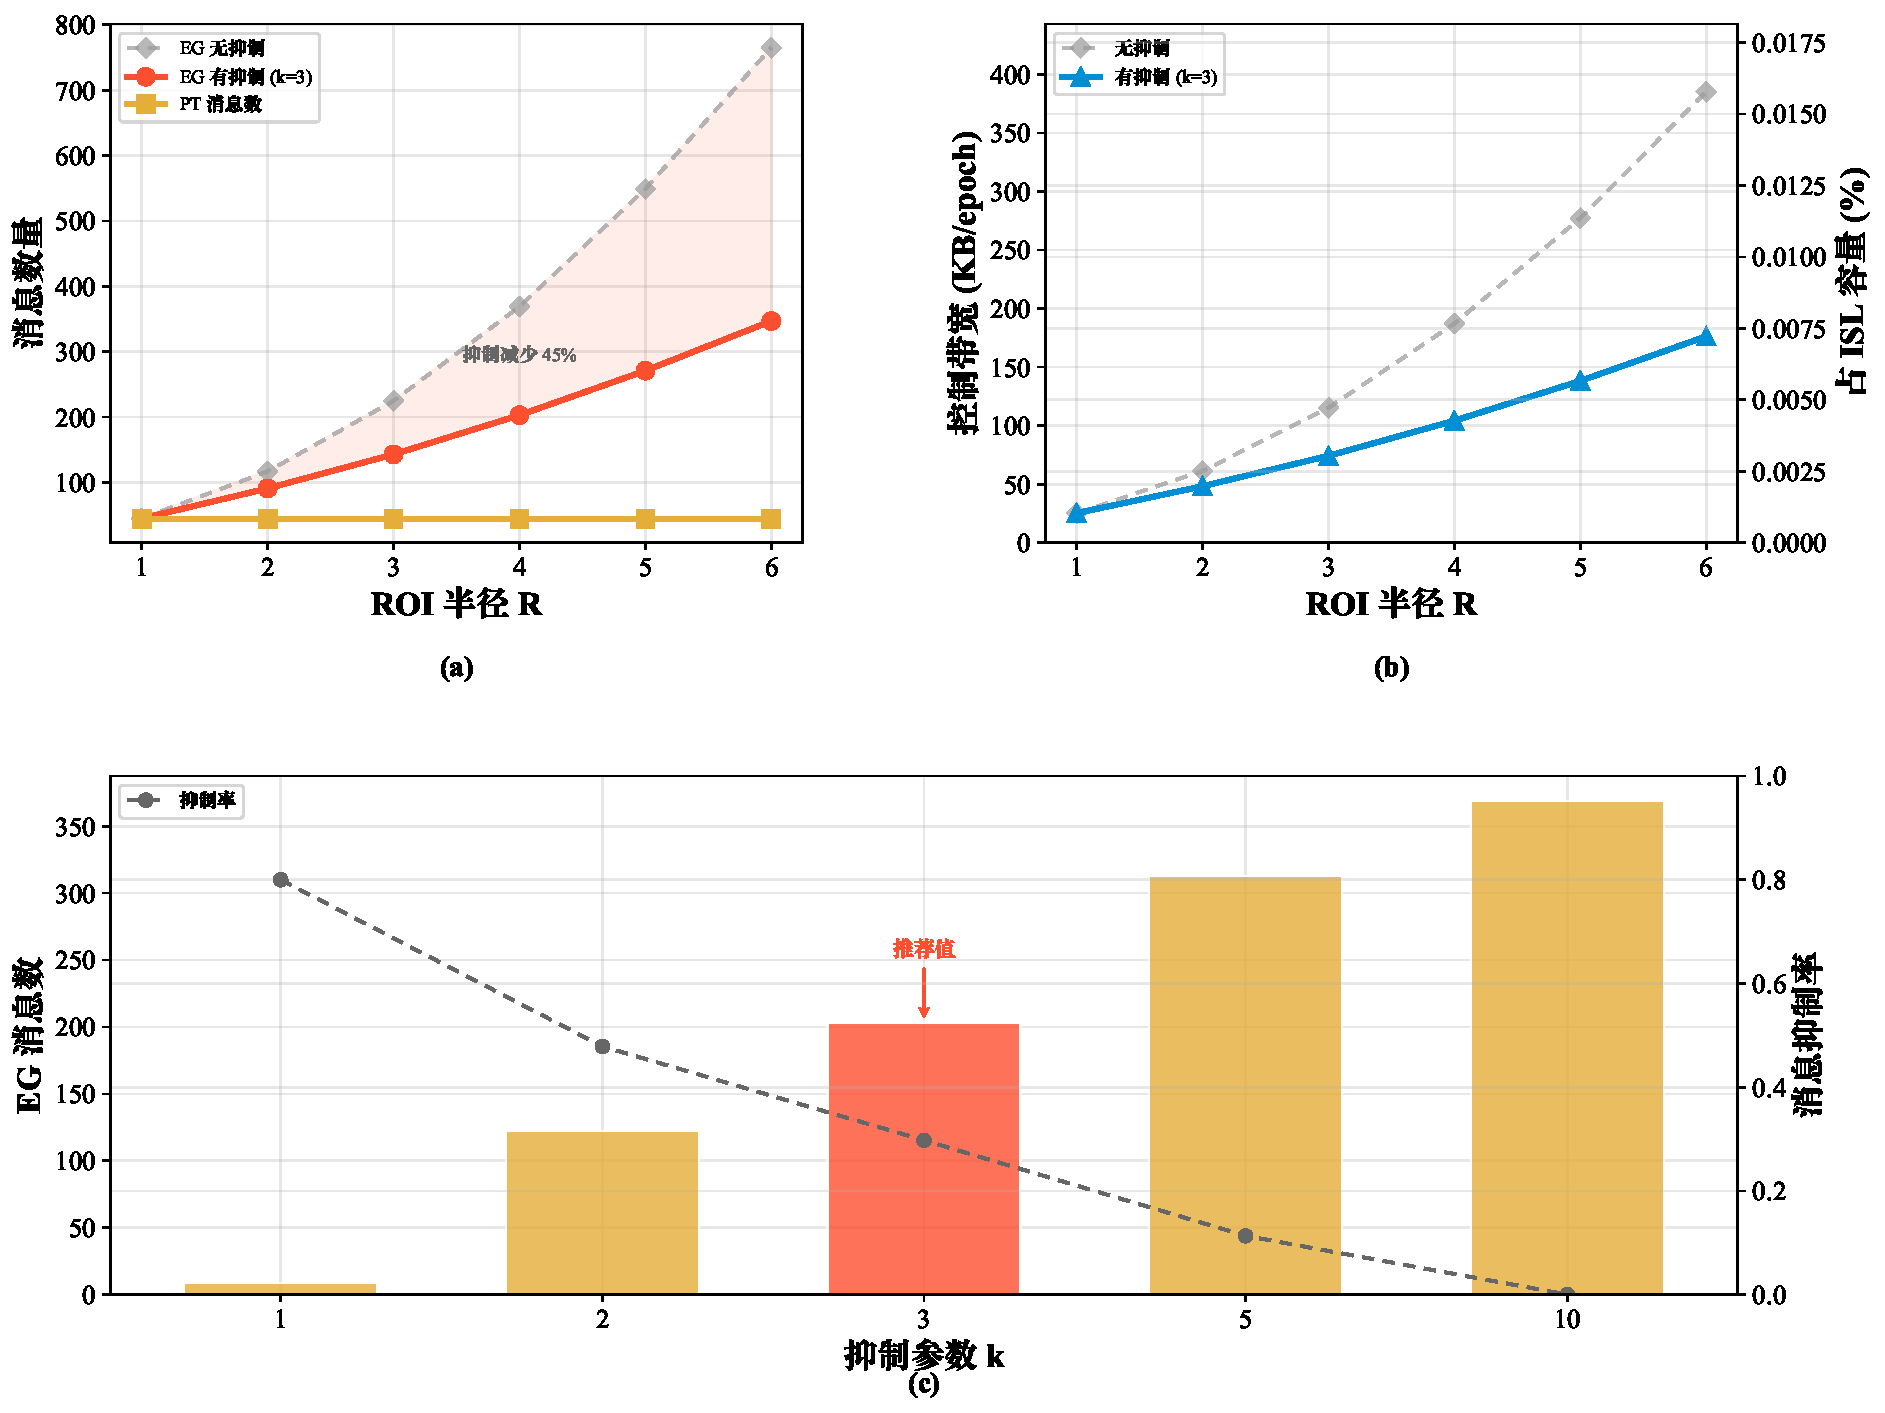
\includegraphics[width=0.92\linewidth]{figs/ch4/fig4_overhead.pdf}
\caption{协同控制开销与抑制机制效果。(a)EG消息数随$R$变化：灰色虚线为无抑制基线，红色实线为有抑制（$k=3$），填充区域为抑制收益；(b)控制带宽随$R$变化，按保守的$n=100$口径统计EG载荷并计入PT总字节，右轴标注占ISL容量百分比（$R=4$时仅$0.004\%$）；(c)抑制参数$k$的影响，$k=3$为工程默认值。}
\label{fig:ch4_ctrl_overhead}
\end{figure}

\subsubsection*{（4）对碎片化攻击证据的鲁棒性}
图~\ref{fig:ch4_robustness}用$2\times2$子图评估了各方案在碎片化攻击（$M\in\{1,5,10,50,100,500,1000\}$）下的表现。四个子图分别给出检测效果（F1 与 Recall）、检测精度（Precision）、良性吞吐恢复以及无效带宽占用。

\textbf{F1 的倒 U 型变化}（子图(a)）：MS-SatShield 与 CoopSatShield 的 F1 随$M$呈现倒 U 型，而不是简单的单调递减，这一变化大致可以分成三段。

当$M\leq10$时，所有方案的 Recall 都保持在$1.0$（虚线所示），说明攻击 key 已被完整捕获；但 F1 仍然偏低，例如$M=1$时约为$0.09$。原因并不在于漏检，而在于存在约 19 个良性重流 key 被持续误判为可疑，这些 key 的聚合速率为$474\sim606$~Mb/s，超过$\tau\cdot\text{rate}_{p99}=242.5$~Mb/s。由子图(b)可见，$M=1$时 Precision 只有$0.05$（TP$=1$，FP$\approx19$），因此 F1 偏低主要是 Precision 不足造成的。这里需要强调，F1 较低并不意味着检测无效：在$M=1$时，唯一的攻击 key（聚合速率$10{,}024$~Mb/s）仍被正确识别，子图(c)也表明 SatShield 与 MS-SatShield 的吞吐都恢复到了$0.886$，CoopSatShield 通过推回则进一步恢复到$1.000$。

当$M=50\sim100$时，攻击 key 数量已经明显多于误报数，FO/FI 特征开始有效地区分攻击流量与良性流量。$M=100$时，MS-SatShield 的 Precision 升至$0.833$，Recall 仍保持$1.0$，F1 达到峰值$0.909$。同一区间内，SatShield 已经完全失效，$M=50$时 F1 仅为$0.057$，$M=100$时进一步降到$0.017$，因为此时攻击 per-key 速率已经接近良性$p_{99}$，rate-only 无法完成区分。这一结果与\ref{chap:ms_satshield}图~\ref{fig:ch3_fig2_f1}(b)中的分离段分析保持一致。

当$M\geq500$时，攻击 key 的单 key 速率降至$20\sim35$~Mb/s，大量 key 脱离 top-$K$候选集（TopK~Recall$\approx0.30$）。MS-SatShield 的 Precision 反而提高到$0.936\sim1.000$，因为被筛入候选集的攻击 key 几乎都能被正确识别，但 Recall 只有$0.30$，最终使 F1 降至$0.445\sim0.466$。

\textbf{CoopSatShield 与 MS-SatShield 的 F1 完全一致}（子图(a)中两条 F1 实线重合）。原因在于二者共享同一检测流水线，即同一个多签名评分器。在当前实验采用的 bot 均匀分布场景下，各节点的本地 top-$K$命中率已经足够高，协同证据聚合不会改变单节点的检测输出。因此，本章协同机制的价值主要体现在缓解层面，而不是检测层面。gossip 负责跨节点共享攻击信息，pushback 则据此把缓解动作从受害链路前推到更上游的入口，这正对应了引言中提出的上游带宽浪费问题。子图(c)显示，在低到中等碎片化范围内，CoopSatShield 的良性吞吐明显高于 MS-SatShield。若统一采用与图~\ref{fig:ch4_throughput}一致的攻击期间稳态平均吞吐口径，则$M\leq 50$时其恢复值接近$1.000$，$M=100$时仍为$0.959$，显著高于 MS-SatShield 的$0.886$；子图(d)则显示，CoopSatShield 的$W_{\text{waste}}$在各个$M$值下都保持最低，这也与图~\ref{fig:ch4_waste_reduction}中的渐进退化分析一致。当$M\geq500$时，所有方案的吞吐都开始退化，CoopSatShield 也下降到$0.80$，反映出候选集覆盖率瓶颈最终会传导到缓解层面。需要补充说明的是，在 bot 分布极不均匀的特定场景下，例如攻击流量集中经过少数中继节点、而这些节点的本地候选集又无法完全覆盖时，协同聚合仍然可能提高检测 Recall；但在本章采用的均匀 bot 分布假设下，这种效果没有显现。

% TODO: 这里的图口径和上一章的图口径不一致，需要统一
% \noindent\textbf{图口径说明。} 若后续重绘图~\ref{fig:ch4_robustness}(c)，建议将$M=100$点调整为与图~\ref{fig:ch4_throughput}一致的稳态平均口径；若沿用当前导出脚本，则应至少在图注中显式注明其统计定义是“恢复峰值”还是“攻击期均值”。

\begin{figure}[!htb]
\centering
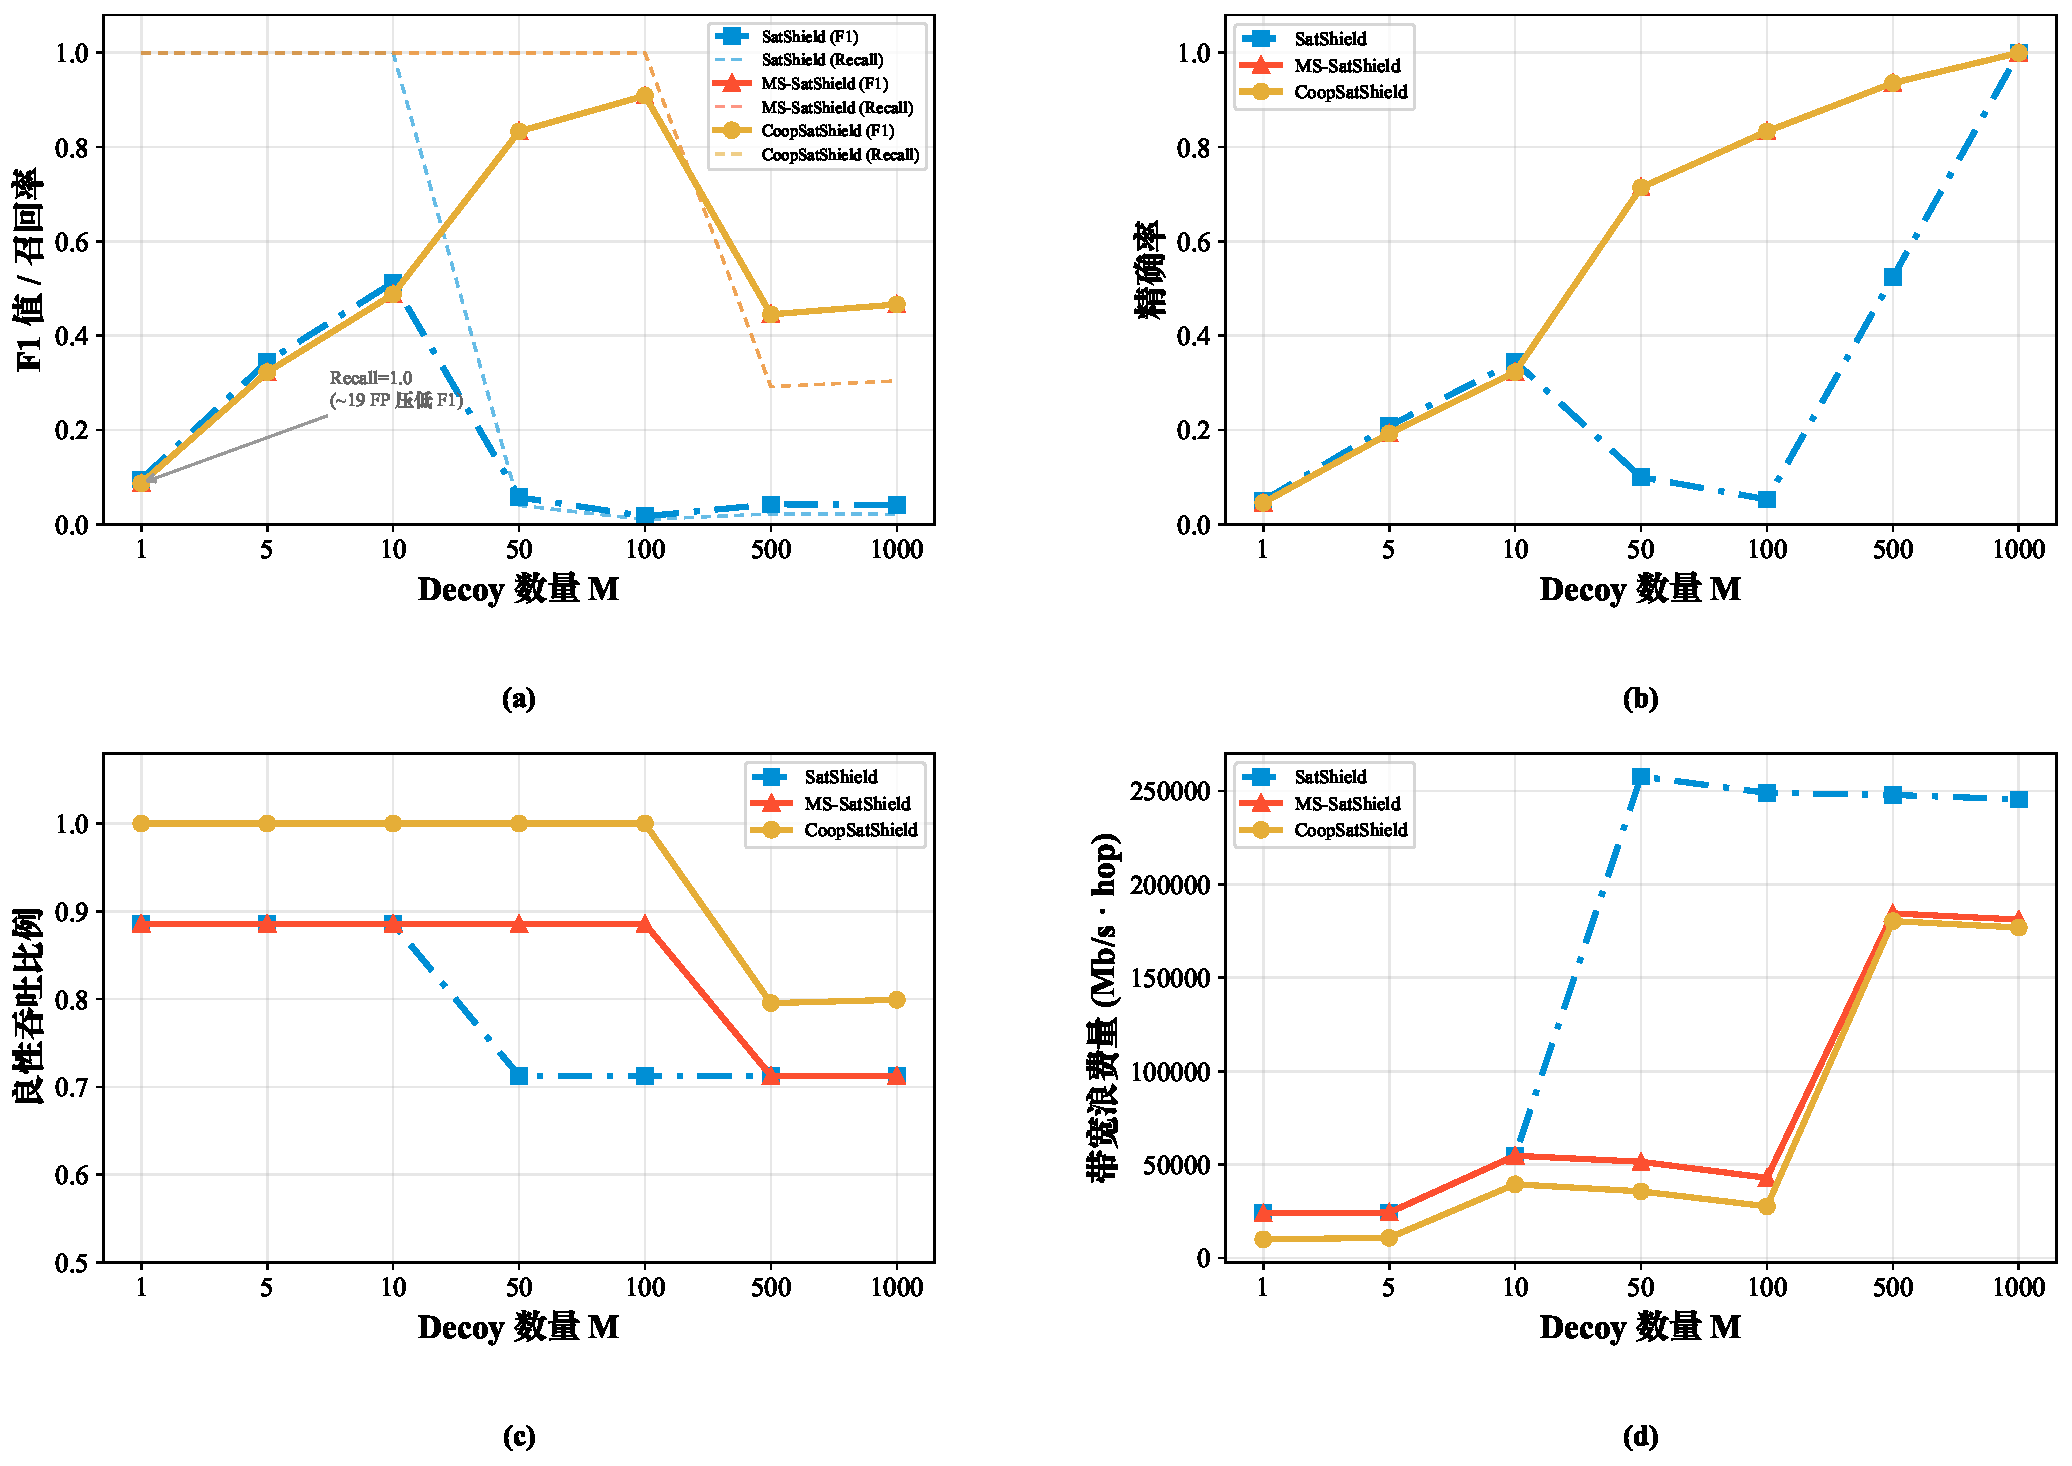
\includegraphics[width=0.92\linewidth]{figs/ch4/fig4_robustness.pdf}
\caption{碎片化攻击下的鲁棒性（$2\times2$子图）。(a)F1（实线）与Recall（虚线）随$M$变化，注意$M\leq10$时F1低是Precision不足所致，Recall始终为1.0；(b)Precision随$M$变化；(c)良性吞吐恢复；(d)无效带宽$W_{\text{waste}}$。}
\label{fig:ch4_robustness}
\end{figure}

\subsection{适用边界与讨论}
\label{subsec:ch4_discussion}

\noindent\textbf{量化比较范围。} 本章正文中的数值比较严格限定在 NoDefense、SatShield、MS-SatShield 与 CoopSatShield 四类星载方案之内。LinkScope、Woodpecker、RADAR、Ripple 与 Mew 等地面 LFA 防御机制仍然有参考价值，但在统一的 LEO 实现完成之前，它们更适合作为设计假设和控制闭环差异的讨论对象，而不适合直接写入本章实验结论。

\noindent\textbf{协同聚合的作用层次。} 在当前均匀 bot 分布设定下，协同聚合评分$S^{\text{net}}$并未改变检测 F1，因此本章能够支持的主要结论是：加权聚合有助于稳定 pushback 触发，但没有表现出显著提高检测能力的作用。若后续需要进一步说明式\eqref{eq:net_score}与式\eqref{eq:weight}相对于简单 avg 或 max 规则的必要性，最直接的办法是补充聚合规则消融以及$\Theta_{\text{pb}},\lambda,\mu$的敏感性实验。

\noindent\textbf{推回覆盖率与候选集瓶颈。} CoopSatShield 在$M=100$时仍只能将稳态良性吞吐恢复到$0.959$，说明近似反向路径推回与局部 ROI 覆盖仍然受制于拓扑分叉和路径不确定性；当$M\ge 500$时，一级候选集覆盖率下降又会进一步把检测瓶颈传导到缓解层面。就本章的证据而言，可以较明确地说明推回能够前移缓解位置并显著降低网络内部成本，但还不能说明它在任意碎片化强度下都能近乎完全消除攻击影响。

\section{本章小结}
\label{sec:ch4_summary}

本章面向大规模低轨卫星网络中的链路洪泛攻击，将研究范围从单星本地闭环防御进一步扩展到多星协同在网计算与推回缓解。针对 LEO 网络中控制环延迟高、拓扑变化快、攻击自适应速度快等约束\citess{satshield,icarus}，本文提出\textsc{CoopSatShield}：在\ref{chap:ms_satshield}的本地多签名检测基础上，将检测输出组织为可协同处理的证据单元；设计抑制型邻居扩散协议，通过事件驱动、ROI 限制和冗余抑制来控制大规模网络中的信令扩散；再结合逐跳 pushback 机制，利用入端口贡献分布实现不依赖全局逆路由的推回缓解，把攻击抑制位置前移到上游入口，从而降低网络内部无效带宽占用并提升良性吞吐保护。

实验结果表明，CoopSatShield 在$M=100$时可将路径积分无效带宽占用成本$W_{\text{waste}}$降至 NoDefense 的$11.0\%$，相比 MS-SatShield（$17.1\%$）再降低$6.1$个百分点；在良性吞吐方面，攻击期间的稳态吞吐维持在$0.959$，相较 MS-SatShield（$0.886$）提升$7.3$个百分点，本地检测与 pushback 的生效时延分别为$T_{\text{det}}=1$~epoch和$T_{\text{pb}}=2$~epoch；在协同开销方面，推荐配置$R=4,k=3$下，按保守$n=100$口径统计的控制带宽仅占 ISL 容量的$0.004\%$，抑制机制还使 EG 消息数比无抑制基线减少$45\%$，没有出现信令风暴；在碎片化攻击场景下，$M=100$时 F1 达到峰值$0.909$，低至中等碎片化范围内良性吞吐接近$1.000$，即使在$M=100$时也仍保持$0.959$。这些结果把全文关于大规模低轨卫星在网计算的研究，从单节点处理自然推进到了多节点协同处理。

\noindent\textbf{局限性与未来方向。} 本章仍有几方面局限。首先，在本章采用的均匀 bot 分布假设下，协同聚合评分$S^{\text{net}}$并未改变单节点检测输出，因此协同的主要收益仍停留在缓解层面，也就是 pushback；在 bot 分布极不均匀或攻击流量集中经过少数中继节点的场景下，协同聚合可能提高检测 Recall，但这一点还需要专门验证。其次，候选集覆盖率仍是主要瓶颈。$M\geq500$时，大量攻击 key 的单 key 速率低于 top-$K$门限而脱离候选集，导致所有方案的 F1 与吞吐保护都开始退化。如何在候选集规模与数据面资源消耗之间找到更合适的平衡，仍有待进一步研究。最后，本章默认所有邻居节点均可信，没有考虑恶意节点注入虚假 EG/PT 消息的情况。针对这类拜占庭攻击，后续可以引入轻量级签名或声誉机制来验证消息；此外，跨轨道面协同以及与 SDN 控制面的混合架构对接，也值得继续展开。
